\documentclass[]{article}
\usepackage{amsmath}
\usepackage[utf8x]{inputenc}
\usepackage{color}
\usepackage{tikz}
\usepackage{graphicx}
\usepackage{subfig}
\usepackage{tikz-cd}
\usetikzlibrary{decorations.pathmorphing}

\usepackage{lineno}

\usepackage[ukrainian]{babel}
\author{Березюк~Іван}
\graphicspath{ {img/} }

\title{ Дипломна робота \\
		Науковий керівник: Олег Анатолійович Безшийко \\
		Науковий керівник(CERN): Massimiliano Ferro-Luzzi\\
		}

\begin{document}
	 \linenumbers
	\maketitle
	\newpage
		
	
 \section{STRAW tubes}
	The option for STRAW tubes is similar as in NA62 experiment with one main difference -- the length is twice longer( $5m$ versus $2.1m$).
	
	The next table. \ref{table:straw_par} describe STRAW tube options.

	\begin{table}[h]
	\centering
	\begin{tabular}{|l|l|p{8cm}|}
		\hline
		Parameter name & Value \\
		\hline
		wire & $30\mu m$ gold-plated Tungsten\\
		\hline
		straw length & $5m$ \\
		\hline
		Voltage & $1750 V$ \\
		\hline
		inner tube radius & $9.8~mm$ \\
		\hline
		wire medium density & $19.3 ~g/cm^3$ \\
		\hline
		Wire tension& $\sim 90~g$ \\
		\hline
		Working tube gas mixture & $Ar70\% ~CO_2 30\%$ \\
		\hline
	\end{tabular}
	\caption[Table caption text]{STRAW tube parameters }
	\label{table:straw_par}
	\end{table}		
	
	\section{Signal}	
	Computer program Garfield \cite{garfield} is designed for detailed simulation of two- and three-dimensional drift chambers. So we will perform STRAW tube studies using this program.
	
	Charged particle  create elector-ion pairs wile traverse the drift tube. Electrons under affecting the electric field drift to the wire anode \ref{fig:track_reconstruction}. During the travel they increase their energy and invoke avalanche. Therefore they produce a measurable signal.

	  Initial electrons drift to the wire due to the electrical field between the wire and the tube wall. Electrons ionize gas molecules due to the high electric field around the wire, especially near the wire when the electric becomes very strong.  Subsequently readout electronics process the signal induced on the wire.
	  
	The event registers if signal reach some a threshold voltage (Fig. \ref{fig:signal_example}). So the value of threshold is a key factor on the way of searching optimal setting for signal processing procedure.
	
	We have to set threshold as low as possible but enough far from noise to achieve highest value of relation true/false detected track and tube efficiency.
		 
	A variation of the signal height introduces a variation in the time when the signal passes the threshold and is considered to be the main contribution to the STRAW tracker resolution.
	
	\begin{figure}[h]
	\begin{tikzpicture}
	
	\tikzset{snake it/.style={decorate, decoration=snake}}
	
	\draw (0,0) circle (4);
	
	\draw[ultra thick] (0,0) circle (0.05);
	\node[below] at (0,0) {wire};
	
	\draw[thick,->] (0,0) -- (1.6,1.6);	
	\node at (1.5,0.7) {$r_{track}$};

	\draw[thick,->] (0,0) -- (-4,0);	
	\node[above right] at (-4,0) {$r_{tube}$};
		
	\draw[thick,->] (-6,2.3) -- (6,2.3);
	\node[above] at (-5,2.3) {$particle$};
	
	\draw[ultra thick, gray, dashed, ->] (-6,-2.3) -- (6,-2.3);
	
	\draw[ultra thick,gray,dashed] (0,0) circle (2.3);
	\node[below] at (3,-2.3) { $r_{rec}$};
	
	% gravitation force vector
	\draw[thick, ->] (-6,1.5) -- ( -6, -1);
	\node[left] at (-6,0) {$\vec{g}$};
	
	% r_track axis
	\node[above,rotate=-90] at (-6,0) {$r_{track}$ axis};
	
	% initial ekectron/ion clusters
	\draw[thick,orange] (-3.0,2.3) circle(0.05);
	\draw[thick,orange] (-2.7,2.3) circle(0.05);
	\draw[thick,orange] (-2.6,2.3) circle(0.05);
	\draw[thick,orange] (-2.5,2.3) circle(0.05);
	\draw[thick,orange] (-2.1,2.3) circle(0.05);
	\draw[thick,orange] (-1.8,2.3) circle(0.05);
	\draw[thick,orange] (-1.0,2.3) circle(0.05);
	\draw[thick,orange] (-0.6,2.3) circle(0.05);
	\draw[thick,orange] (-0.5,2.3) circle(0.05);
	\draw[thick,orange] (0.26,2.3) circle(0.05);
	\draw[thick,orange] (0.4 ,2.3) circle(0.05);
	\draw[thick,orange] (1.3 ,2.3) circle(0.05);
	\draw[thick,orange] (1.56,2.3) circle(0.05);
	\draw[thick,orange] (1.96,2.3) circle(0.05);
	\draw[thick,orange] (2.22,2.3) circle(0.05);
	\draw[thick,orange] (2.48,2.3) circle(0.05);
	\draw[thick,orange] (2.68,2.3) circle(0.05);
	\draw[thick,orange] (2.88,2.3) circle(0.05);
	\draw[thick,orange] (3.00,2.3) circle(0.05);
	
	\draw[red,snake it](-0.6,2.3) -- (0,0);
	\draw[red,snake it](-0.5,2.3) -- (0,0);
	\draw[red,snake it](0.26,2.3) -- (0,0);
	\draw[red,snake it](0.4,2.3) -- (0,0);
	\node[] at (-0.3,1) {drift path};
	
	\end{tikzpicture} 
	\caption{Schematic view of a particle passing the straw and producing
ionization clusters. The ionization cluster electrons drift to the wire and
induce the signal. Only the earliest signal is detected. The closest distance
from the track to the wire, $r_{track}$, and radius of the straw, $r_{tube} = 2.45 mm$, are also indicated.}
	\label{fig:track_reconstruction}
	\end{figure}


	In the track reconstruction software(GARFIELD \cite{garfield} an effective TR-relation is used. It only describes the relation between the drift time and the distance from the track to the wire, which differs from the distance to the ionization cluster. The shape of the TR-relation is defined by the drift velocity of the ionization cluster inside the straw. The electric field increases towards the wire, leading to a non linear TR-relation. Currently almost parabolic dependence is used, and easily can be fitted by function (\ref{eq:fit_tr}).

	The drift time versus the unbiased distance distribution and the result of the fit are shown in Fig. \ref{fig:t_r_distr_00}. Noise hits under the main distribution, i.e. at earlier times, are due to primary or secondary particles ($\delta$-rays) passing the straw at a closer distance to the wire, consequently producing an earlier signal.
	
	Muon $\mu$ was chosen as test particle for simulation with energy $1GeV$. You can see some of typical tracks from the $\mu$ through the tube Fig.\ref{fig:electron_ion_track},\ref{fig:electron_ion_track_sag}. Initial clusters along the track are marked by orange points on the figure.
			
	
	\subsection{ Leakage noise}
	Every time we deal with different kind of noise. Basically it is noise from  leakage current through readout electronics.

	As will be discussed further we analyse not the current invoked by particle but the output voltage from amplifier. In GARFIELD we able convolute input current $I(t)$ with electronic response function (\ref{eq:responce_function}): 
	\begin{equation}
	f_{resp} =  A\cdot(e^{-t/0.005} - e^{-t/0.030})
	\label{eq:responce_function}
	\end{equation}
	
	Noise is very important for every calculations and it makes bit impact on straw precision and straw efficiency. So we can't rely on results until we receive signal and noise  from real STRAW tube prototypes.
		
	Convolution smooth input current. Experiments that used to drift tubes (such as \ref{}(advise of Iouri Guz)) say that the noise should have gauss distribution with RMS equal to a amplitude of signal from 2000 electron in the tube - electric noise charge (ENC). (\textcolor{red}{This part should be clarified more precisely. Would be good to include some results from noise measurements from STRAW tube samples}. In fig.\ref{fig:signal_example} you can see deposition from noise marked by blue line.

On the figure fig.\ref{fig:signal_example} The time stamp $Time=0$ correspond to the time muon cross tube. The convolution function smooths and spreads input current. It mean that the output voltage in GARFIELD does not contain part of signal before hit event time stamp. 

	\begin{figure}[h!]
	\centering
	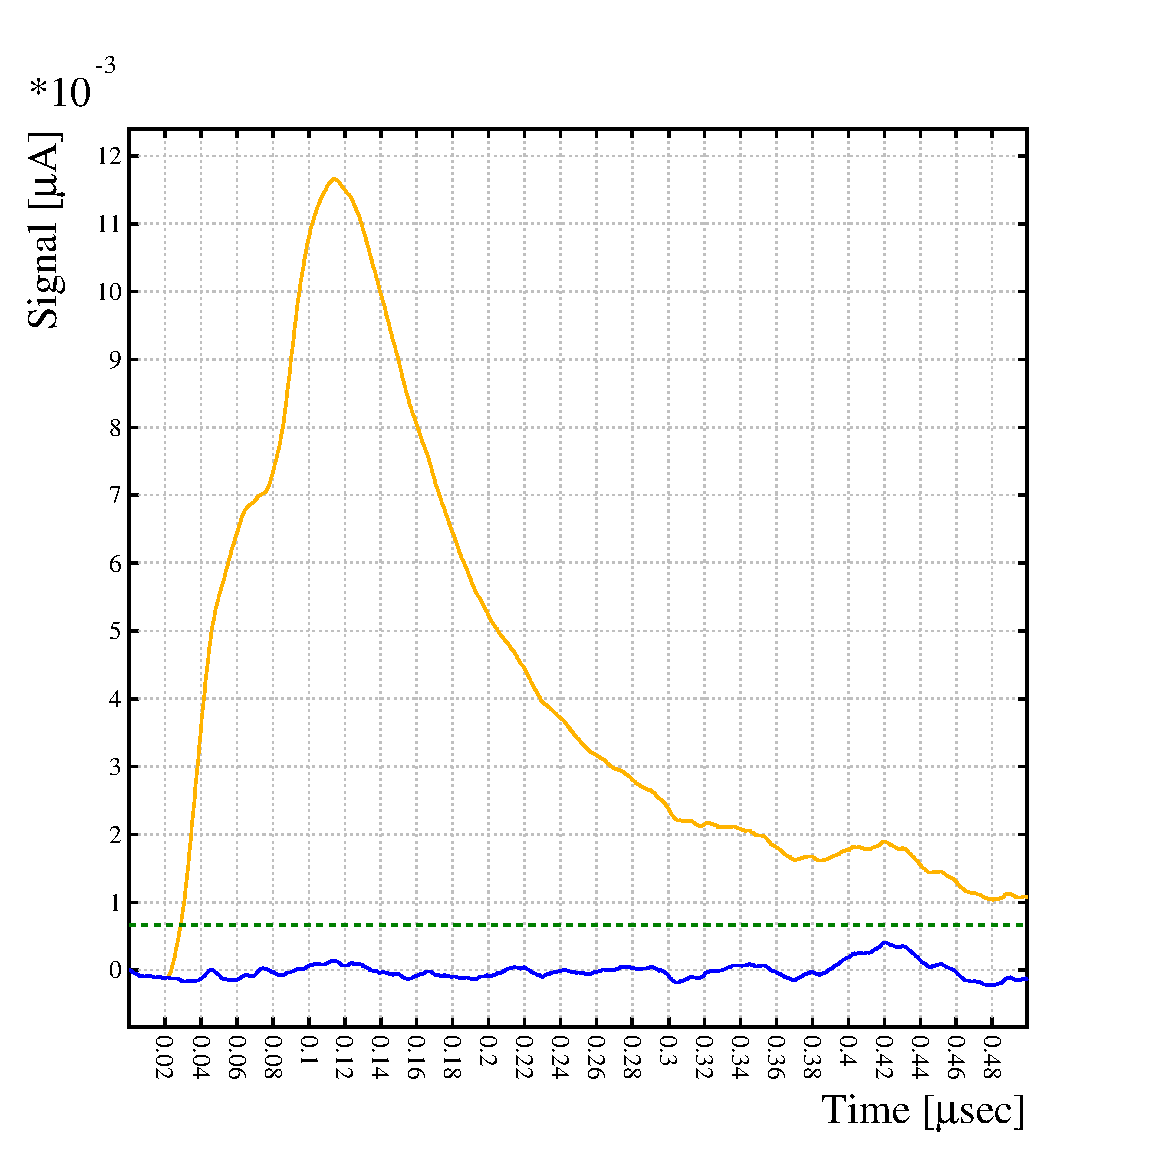
\includegraphics[width=0.7\textwidth]{signal_noise_threshold.eps}
	\caption{ Example of output signal $V(t)$ after convolution(front-end electronics) from central track(yellow line). The noise component of the same signal depicted by separate blue line. Grin dashed line is a threshold for trigering drift time and equal to $5\sigma$ of noise distribution.}
	\label{fig:signal_example}
	\end{figure}
	
	\subsection{ STRAW efficiency}
	
	The interaction of charge particle with gas molecules nave probabilistic nature. For short distance tracks(somewhere at the tube periphery) the probability of tracks that do not produce any electron/ion pair becomes significantly high.
		
	The number of produced ionization clusters directly affects the hit efficiency profile. \cite{kozlinskiy} Smaller ionization length increase hit efficiency because of more ionization clusters per length unit are producing. In GARFIELD we can easily calculate amount of clusters per track. In fig. \ref{fig:cluster_distrib} you can see a distribution of number of clusters per central track for our STRAW tube. It mean that straw efficiency will be lower at the tube wall( see fig. \ref{}).
		

	\begin{figure}[h!]
	\centering
	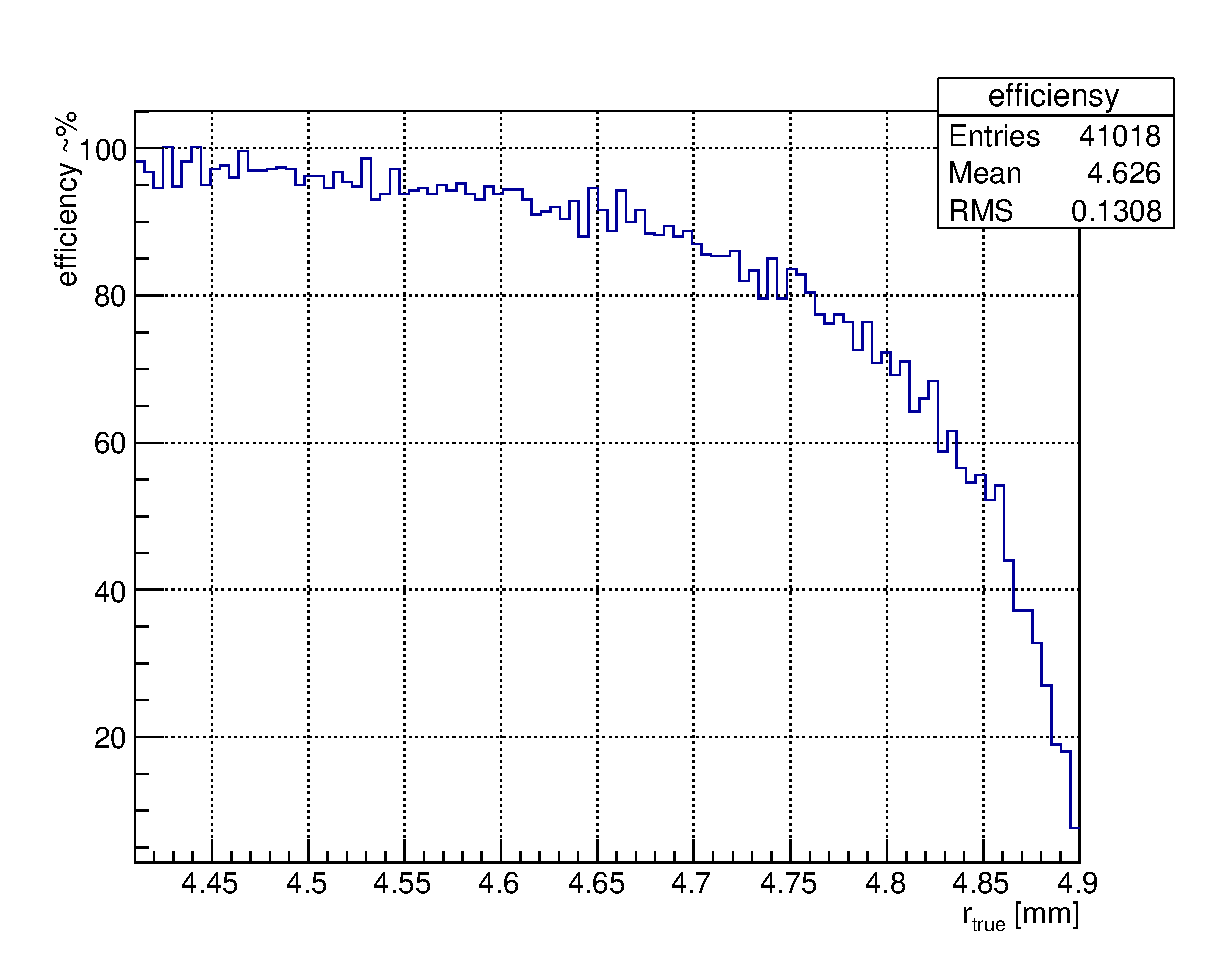
\includegraphics[width=0.8\textwidth]{periffEff}
	\label{fig:efficiency}
	\caption{ Straw tube efficiency. Result of homogeneous penetrating periphery of tube by 50k events(scaled down by factor of 5. $\dfrac{50k~events}{100 bin}  = 500 \dfrac{eventst}{bin}$).}
%	Ефективність реєстрації треків в області периферії трубки від рівномірного опромінення 50 тис. треків
	\end{figure}	
	
	\begin{figure}[h!]
		\centering
		\subfloat[electrons per cluster]{
			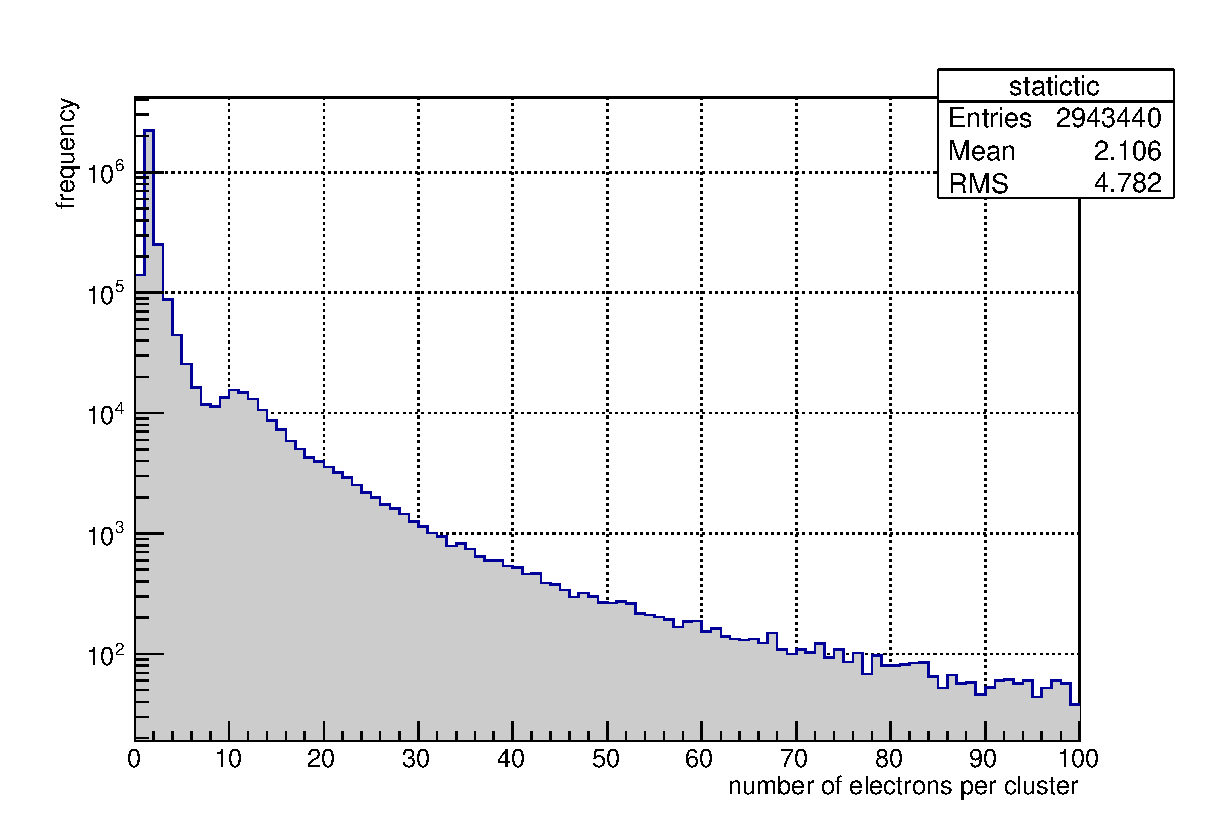
\includegraphics[width=0.45\textwidth]{el_per_cluster} 
			\label{fig:el_per_cluster} }%
		\qquad
		\subfloat[number of clusters per central track]{
			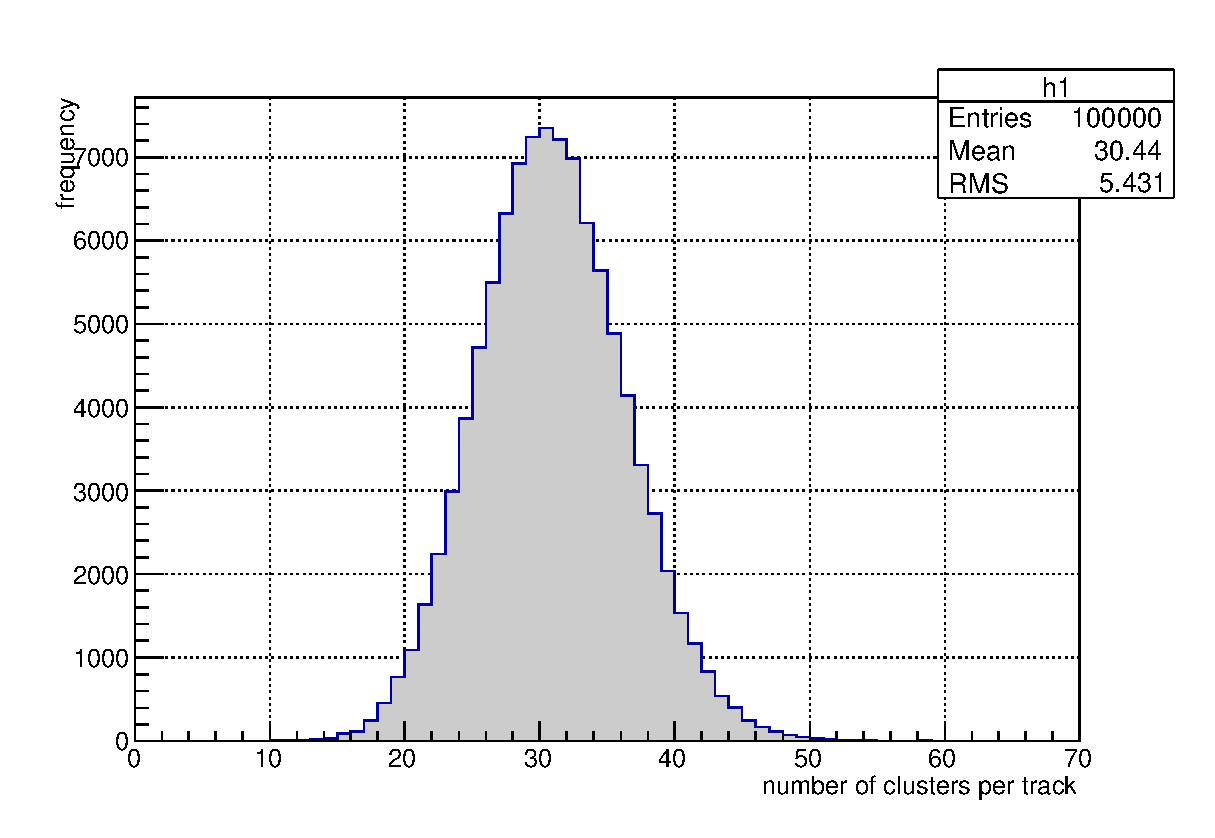
\includegraphics[width=0.45\textwidth]{cluster_distrib} 
			\label{fig:cluster_distrib} }%
		\caption{ \textcolor{red}{ There are big amount of graphs. So I'm trying to pair it. ere we can write something if needed. Some common description of (a) and (b) figures?} }
	\end{figure}
	
	From the figure \ref{fig:efficiency} we can conclude that the efficiency of tube is $100\%$ almost in whole region covered by tube except pre wall region which is quite small. Increasing the gas mixture density or increasing the tube radius for the same gas density can increase tube efficiency. Have to check this in feature studies.
		 
	\section{Gain}
	
	If multiplication occurs, the increase of the number of electrons per path $ds$ is given by
	
	\begin{equation}
		dN = N \alpha ds
		\label{eq:diffGain}
	\end{equation}
	
	The coefficient $\alpha$ is determined by the excitation and ionization cross sections of the electrons that have acquired sufficient energy in the field. It also depends on the various transfer mechanism and electric field E and increases with the field because the ionization cross-section goes up from threshold as the collision energy $\varepsilon$ increases. As we can suppose the coefficient $\alpha$ is of big amount of parameters.
	
	The amplification factor $G$ on a wire(that is more interesting for us) is given by integrating (\ref{eq:diffGain}) between the point $s_{min}$ where the field is just sufficient to start the avalanche and the wire radius $a$:
	
	\begin{equation}
	G = N/N_0 = exp \int\limits_{s_{min}}^{a} \alpha(s) ds
	\end{equation}
	
	GARFIELD can provide us by amplification factor $G$ for any point of the tube(because  $G$ is coordinate dependent magnitude). The amplification factor is equal almost in whole tube space except neighbourhood near the wire because electric field  becomes significantly high only near the wire (see figs \ref{fig:elFieldCentered}, \ref{fig:elField1mmShifted}). When the wire is shifted from the center of the cube the electric field in area close to the wire is the same as in centered state. So the amplification factor $G$ is quite similar in both cases.
	
	\begin{figure}[h!] 
		\centering
		\subfloat[electric field for centered wire]{
			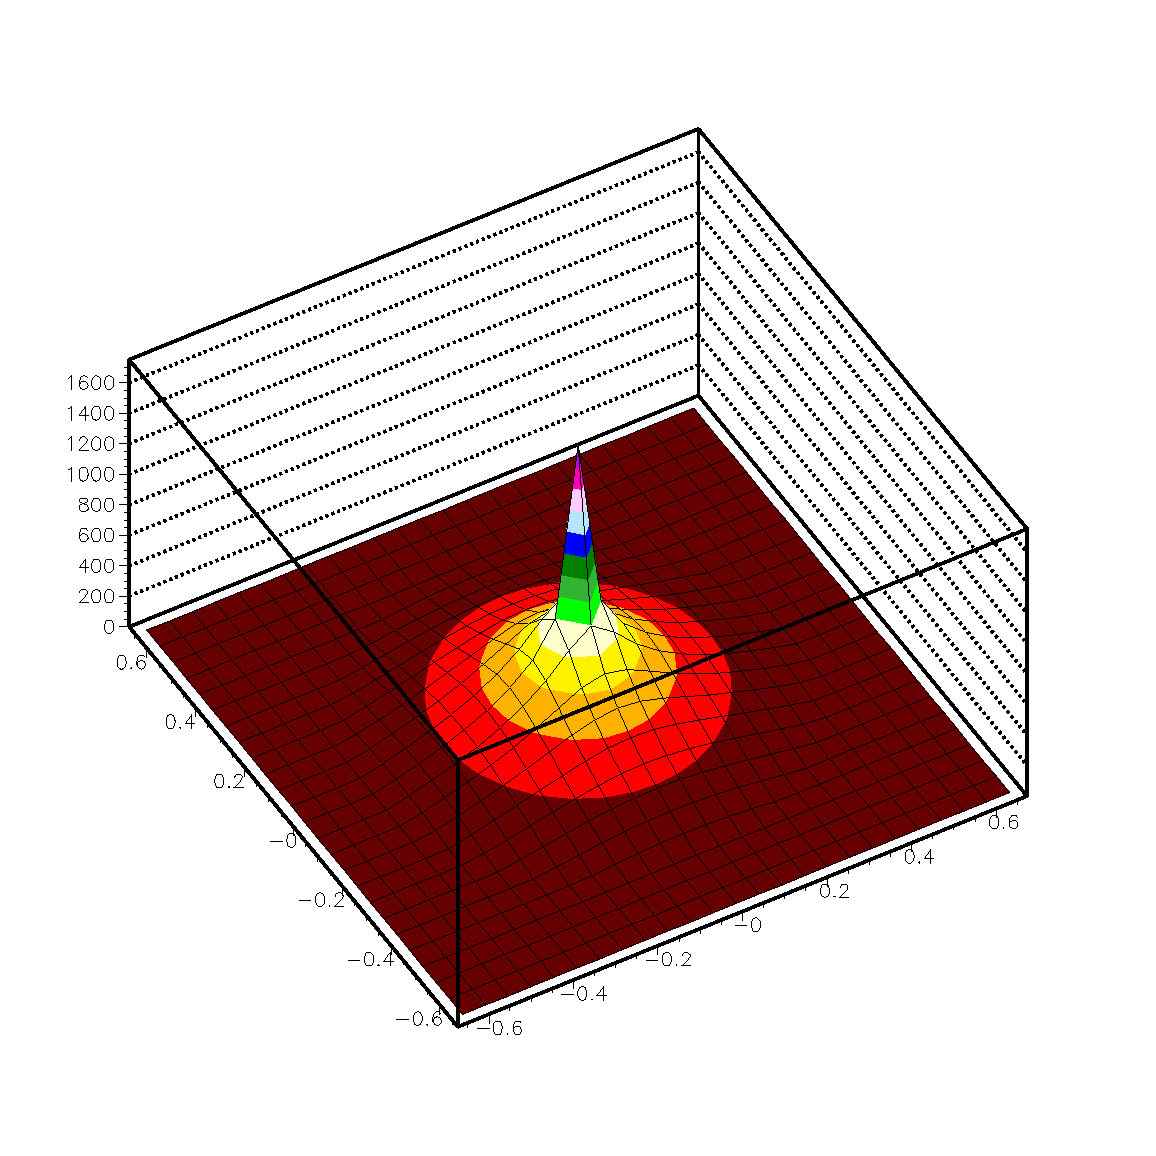
\includegraphics[width=0.45\textwidth]{fieldCentered} 
			\label{fig:elFieldCentered} }%
		\qquad
		\subfloat[electric field for $1 mm$ shifted wire]{
			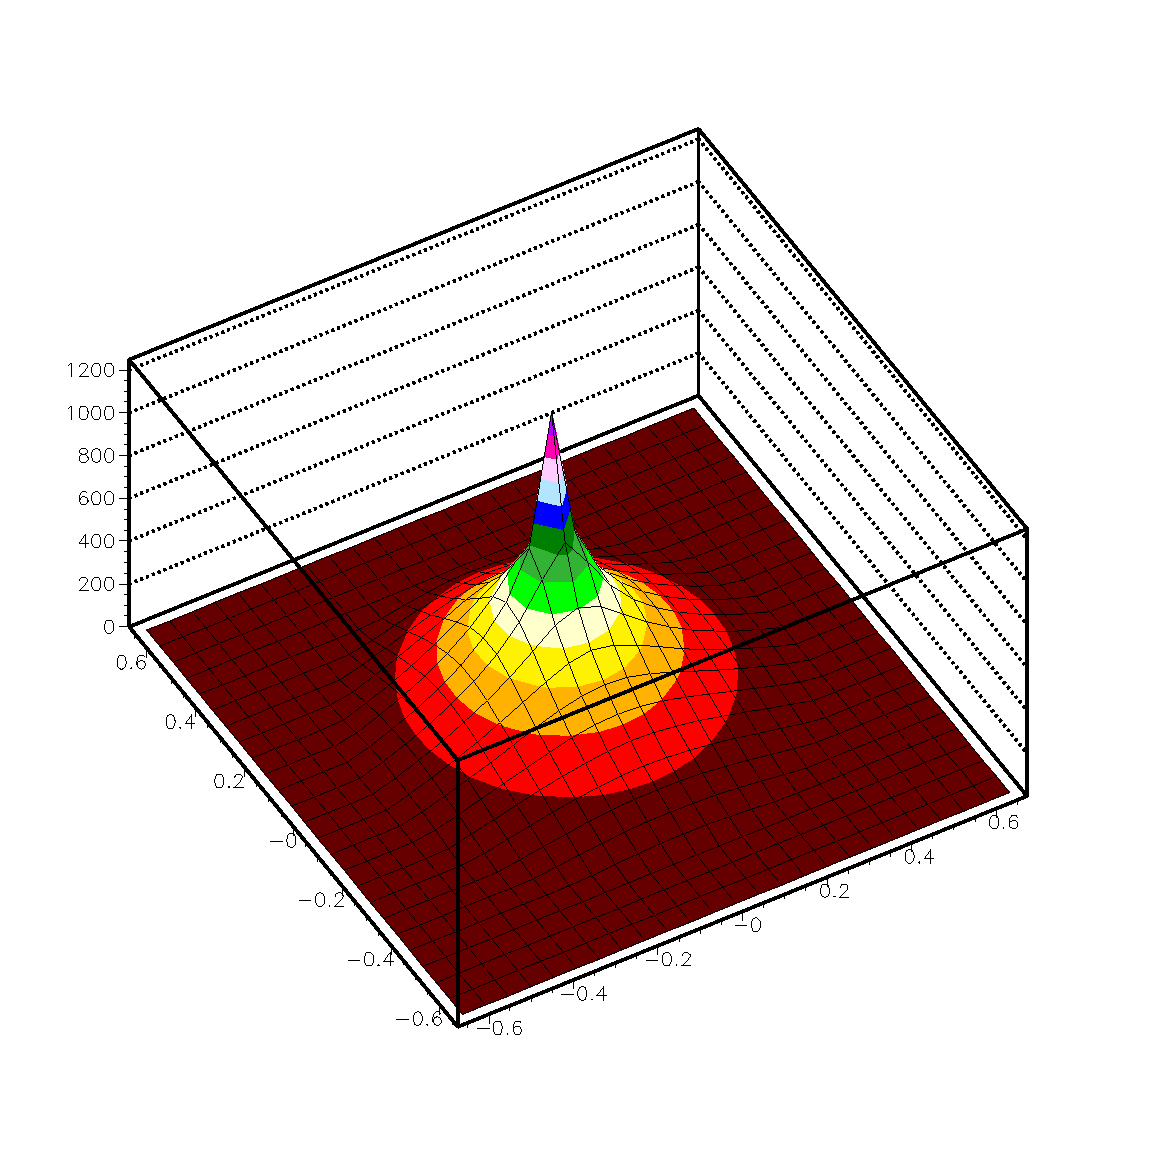
\includegraphics[width=0.45\textwidth]{field_10Sag}
			\label{fig:elField1mmShifted} }%
		\caption{Electric field intensity map for different wire position in the cube calculated in GARFIELD software. Conditions for those plots are described in table \ref{table:straw_par} }
	\end{figure}
	
	Implementation of gain value calculation is not so reliable in GARFIELD(especially fortran version). So we can reach better results using Garfield++ (which is newer and take into consideration more effects).

	On the Fig.~\ref{fig:gain-voltage-dendence} you can see that the gain $G(V)$ have precisely exponential dependence. This is frankly does not inspire confidence. The difference can be up to 100\% (us Rob Veenhof\cite{garfield} said).
	
	\begin{figure}[h!]
	\centering
	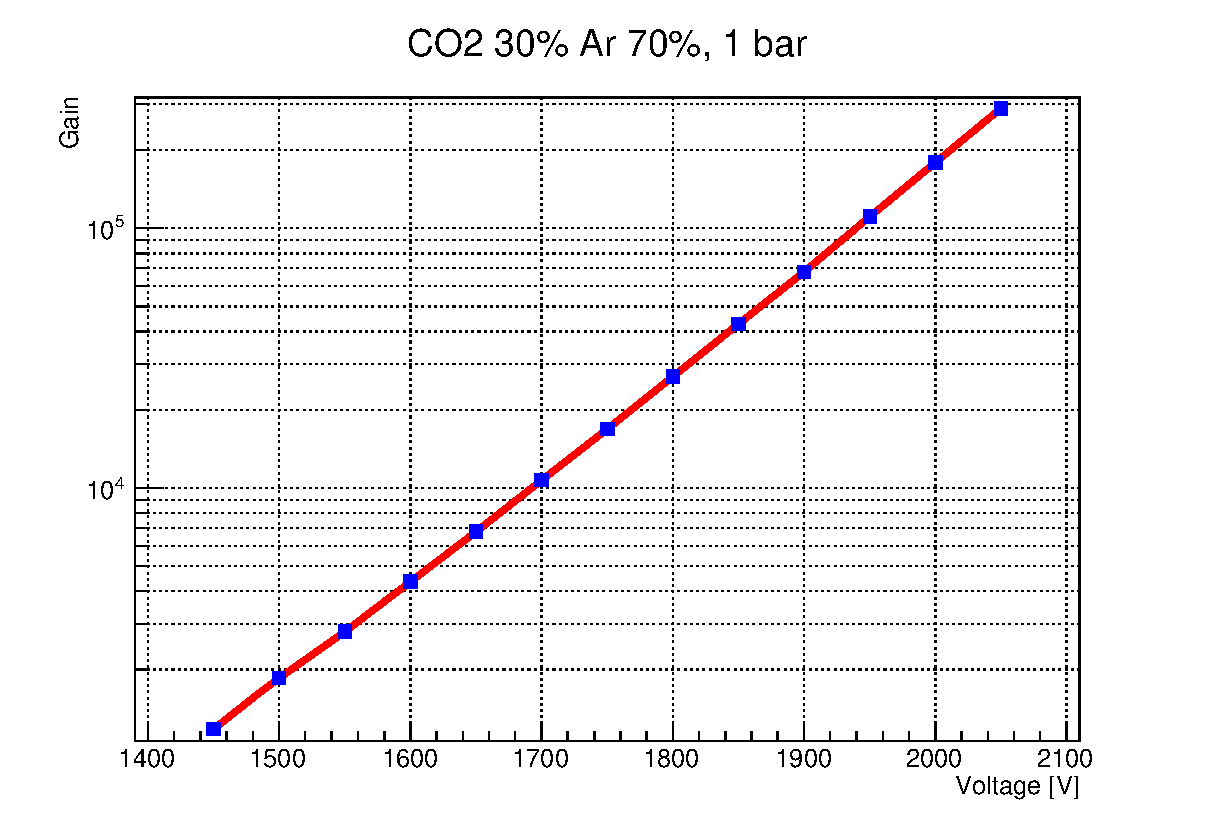
\includegraphics[width=0.8\textwidth]{gain_1450_2050V}
	\label{fig:gain-voltage-dendence}	
	\caption{Dependence of the gain of the voltage applied to the wire. The rest of STRAW tube settings you can find in table \ref{table:straw_par}. \textcolor{red}{need add gain(v) graph for shift wire STRAW tube for comparison} }
	\end{figure}
	
	\section{ Wire sagging}
	Easy to predict that the shifting of the wire invoke distorting an electric field(see figs~\ref{fig:elFieldCentered},\ref{fig:elField1mmShifted}) and drift path for electrons/ions inside the tube(see fig.\ref{fig:electron_ion_track} and fig.\ref{fig:electron_ion_track_sag}). The rt-relation for track reconstruction directly depend on the wire position in the tube. So rt-relation lose it's previous symmetry(see next sections).
	
	\begin{figure}[h!]
		\centering
		\subfloat[wire in the center of the tube]{
			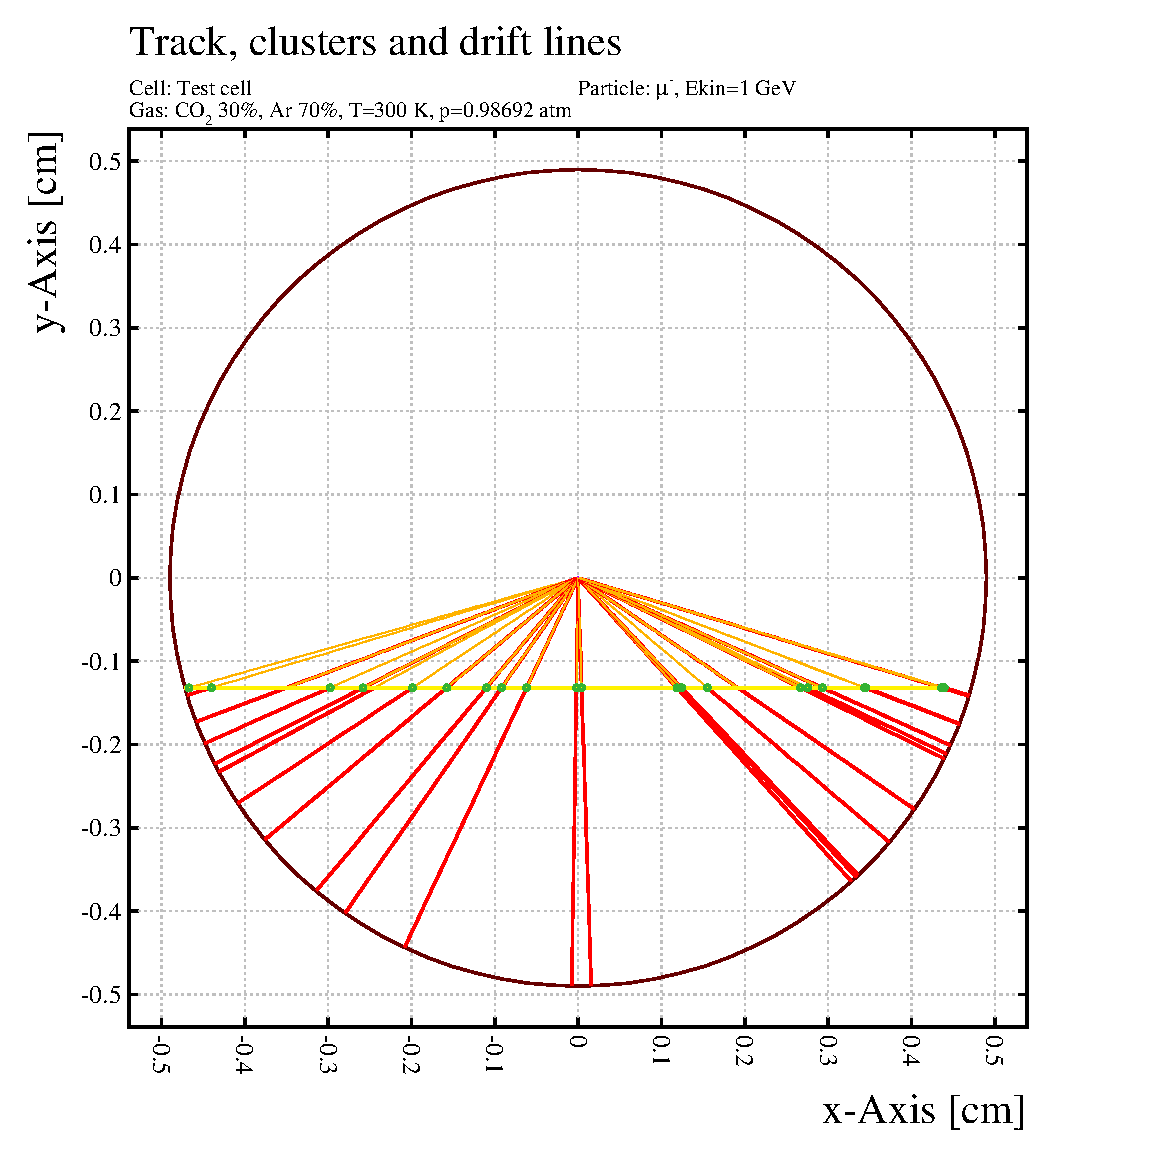
\includegraphics[width=0.45\textwidth]{tracksAndClusters00Sag.eps} 
			\label{fig:electron_ion_track} }%
		\qquad
		\subfloat[sagging $1.5 mm$]{
			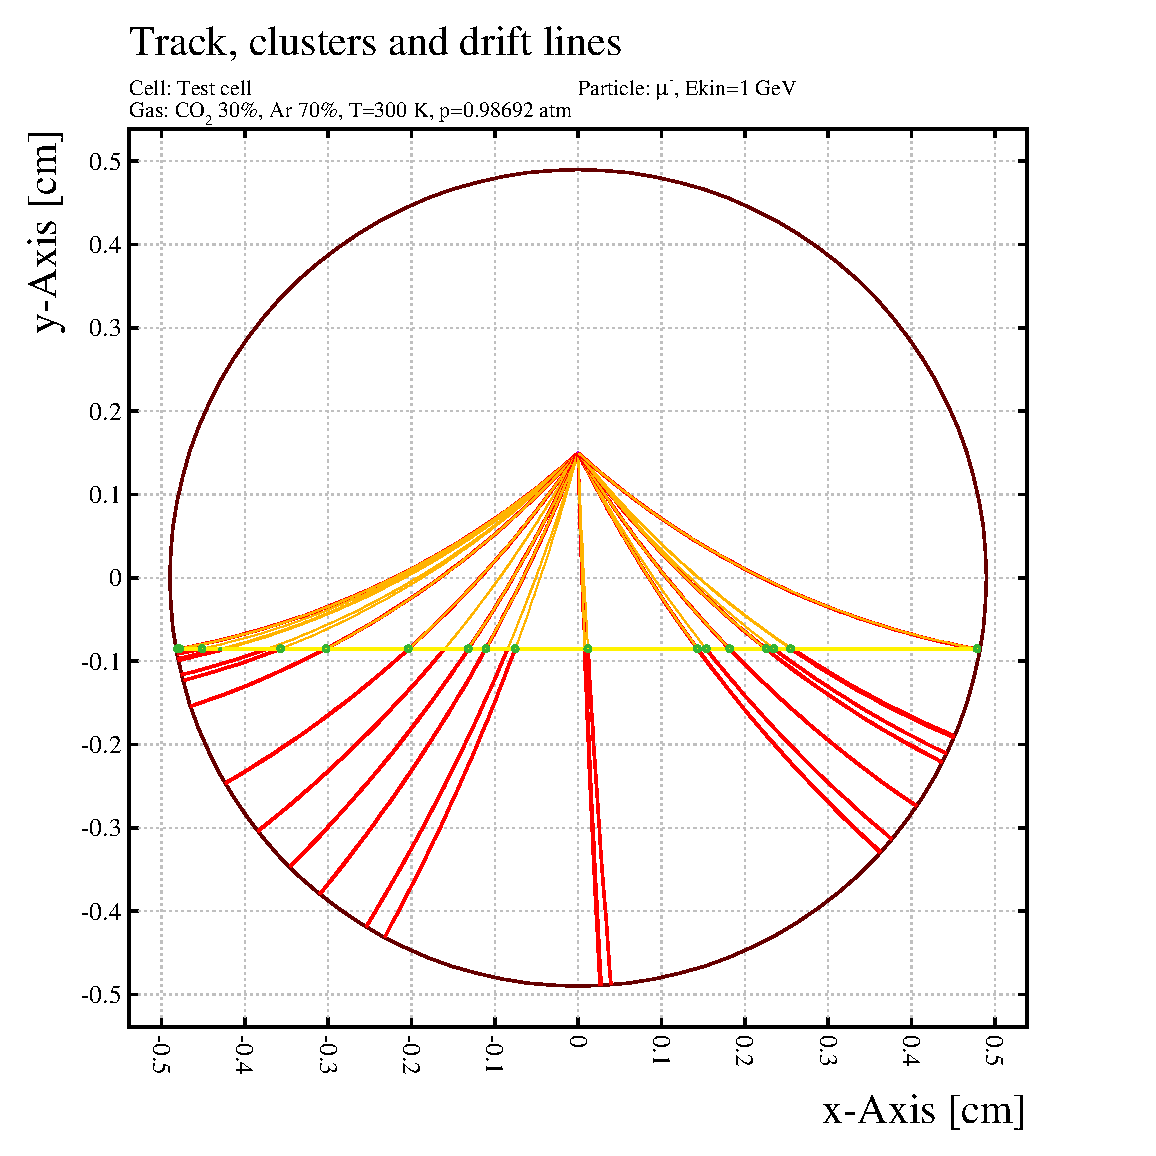
\includegraphics[width=0.45\textwidth]{tracksAndClusters15Sag.eps} 
			\label{fig:electron_ion_track_sag} }%
		\caption{ An example of tracks from the on the tube for different position of the wire from GARFIELD simulations. Initial clusters marker by green. Drift lines for electrons marked by yellow, ions -- red lines.}	
	\end{figure}
	
	The direction of sagging is unpredictable when the wire is centered and the straw has vertical orientation. Impact of gravitation field into the wire does not make any effect in this state. But we can avoid this ambiguity by setting straws horizontally. This condition is necessary to make track reconstruction possible.
	
	We estimate significant wire sagging(by comparison to the tube radius) because of wire attracts to the tube under affecting of gravitation and electric field force.
	
	You can see a profile of wire sagging of $5m$ length wire in $1cm$ diameter straw tube and 1750V voltage on the fig.\ref{fig:sagProfile} calculated in GARFIELD software \cite{garfield}.
	
	\begin{figure}[h!]
	\centering
	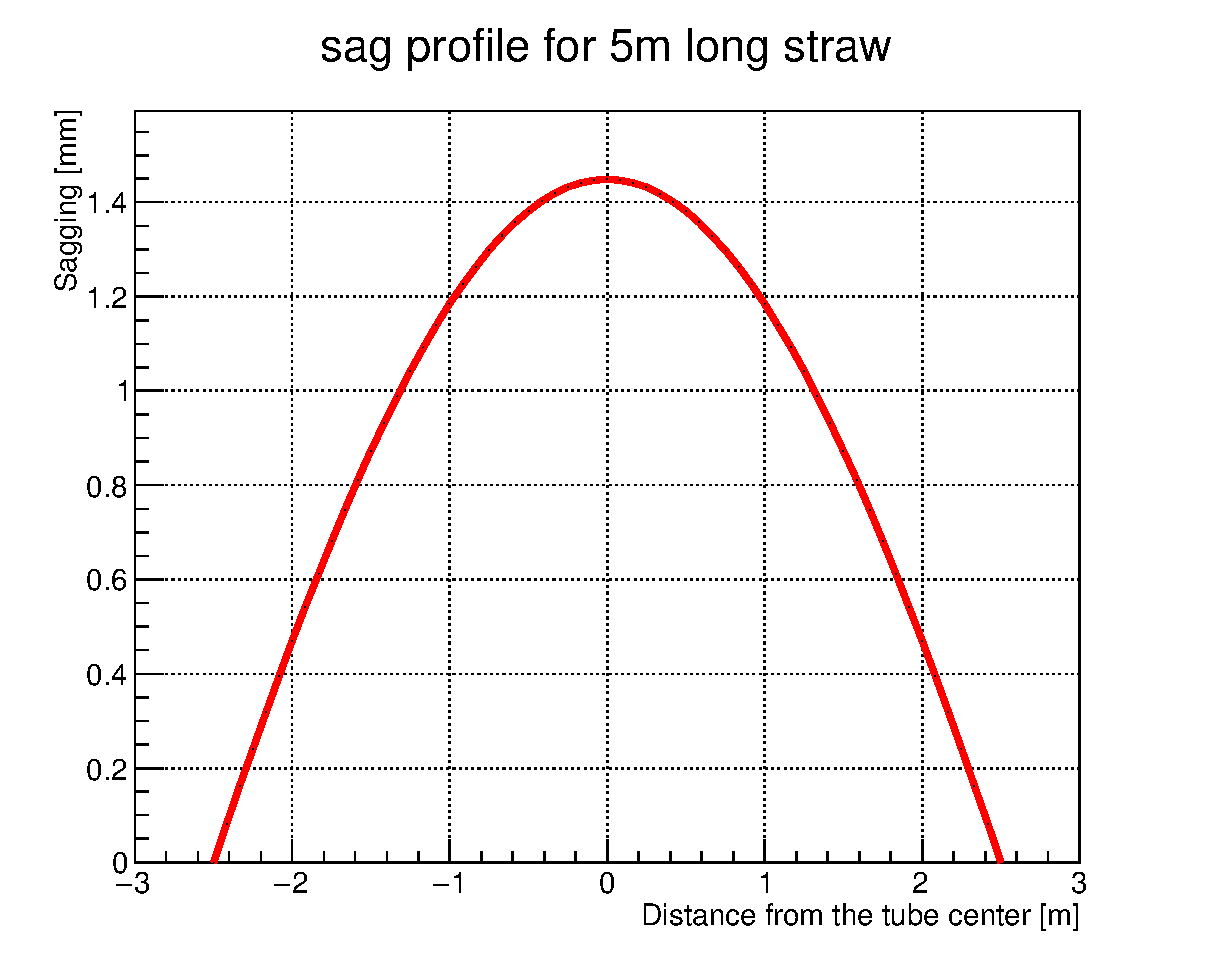
\includegraphics[width=0.7\textwidth]{sagProfileFit.eps}
	\caption{Wire sag profile under electric and gravitation field calculated in GARFIELD. All options for this straw system are described in table~\ref{table:straw_par}.}
	\label{fig:sagProfile}
	\end{figure}	
	
	The calibration of STRAW tube with sagged wire is more difficult by comparison to the mode without sagging. 
	
	Variation of wire tension, wire radius should be taken into account as high affect factor for sag value.
	
	\section{Sag estimation}

	In this section we have to find out method for assessing sagging. This is key step that makes track reconstruction procedure possible.
	
	At first we have to think on data we can use for such kind of calculations. Much attractable information we can extract from drift time distribution. 
	
	The wire sags under electric and gravitation force. Therefore the sag value is differ along the tube(fig~\ref{fig:sagProfile}). But we can separate collected data for different position along the tube. STRAW tube detector consist of several parallel layers of tubes at some angle to each other. So we can easily fix longitudinal position  for tracks that cross several crossed tubes(at least two). Collimation is also possible via scintillator triggering before and after STRAW tube.
	
	Lets say we can install our STRAW tube into homogeneous particle flow and save drift time distribution for some narrow section of the tube. These distributions are different from each other(see example on Figure \ref{fig:DrftTimeDistr_00_09_comp}). The difference between diagrams increasing with sag difference. So it is good possibility for sag calibration.
		
	\begin{figure}[h!]
	\centering
	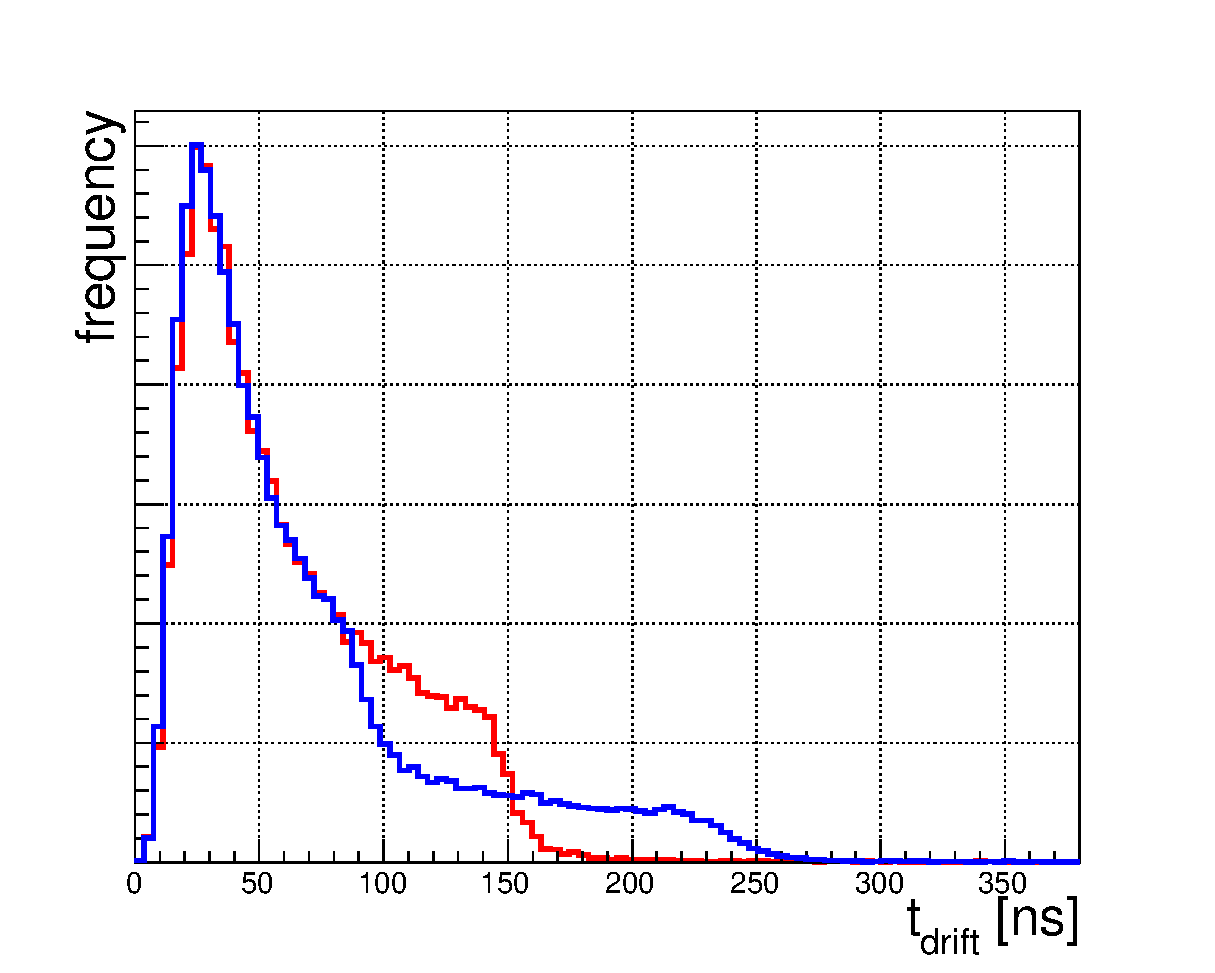
\includegraphics[width=0.8\textwidth]{00_09_driftTimeDistr}
	\label{fig:DrftTimeDistr_00_09_comp}
	\caption{Drift time distribution for a homogeneous irradi-
ation with a centered wire (red) and for a wire offset of 0.9 mm (blue).}
	\end{figure}
	
	Then we have to bind each drift time distribution with appropriate sag value. This is part of laboratory work when sag profile measurements can be performed via optical method prior to the exposition.
	
	Distributions on graph~\ref{fig:DrftTimeDistr_00_09_comp} contain GARFIELD simulations for some certain wire(not for section of sagged wire)because of GARFIELD can handle only two-dimensional tasks.
	
	Lets say we have an equipment for scanning the tube to measure wire sagging profile. After profile measurements we divide our tube into sections. Wire position within separate section should be within desired precision.
	
	So we need divide our tube into $57$ sections (see figure~\ref{fig:tube_sectioning}) if maximum of wire offset(at the center of the tube) is equal to $1.45mm$ and desired precision is $50\mu m$.
	
	\begin{equation}
	N_{halftube} = \frac{1.45 mm}{50 \mu m} = 29;
	\label{eq:tube_sectioning}
	\end{equation}
	
	\begin{figure}[h!]
	\centering
	\begin{tikzpicture}[xscale=0.05,yscale=1]
	
	\tikzset{snake it/.style={decorate, decoration=snake}}
	\draw[snake it,dashed] (0,0) -- (0,1);
	
	\draw[thick] (0,0) -- (250,0) -- (250,1) -- (0,1);
	\draw[] (43.2339,0) -- (43.2339,1) -- 
	(61.2704,1) -- (61.2704,0) -- 
	(75.2004,0) -- (75.2004,1) -- 
	(87.0213,1) -- (87.0213,0) -- 
	(97.5056,0) -- (97.5056,1) -- 
	(107.049,1) -- (107.049,0) -- 
	(115.885,0) -- (115.885,1) -- 
	(115.885,1) -- (115.885,0) -- 
	(124.169,0) -- (124.169,1) -- 
	(132.005,1) -- (132.005,0) -- 
	(139.472,0) -- (139.472,1) -- 
	(146.627,1) -- (146.627,0) -- 
	(153.516,0) -- (153.516,1) -- 
	(160.176,1) -- (160.176,0) -- 
	(166.636,0) -- (166.636,1) -- 
	(172.921,1) -- (172.921,0) -- 
	(179.05,0) -- (179.05,1) -- 
	(185.043,1) -- (185.043,0) -- 
	(190.913,0) -- (190.913,1) -- 
	(196.674,1) -- (196.674,0) -- 
	(202.338,0) -- (202.338,1) -- 
	(207.915,1) -- (207.915,0) -- 
	(213.414,0) -- (213.414,1) -- 
	(218.844,1) -- (218.844,0) -- 
	(224.212,0) -- (224.212,1) -- 
	(229.527,1) -- (229.527,0) -- 
	(234.793,0) -- (234.793,1) -- 
	(240.018,1) -- (240.018,0) -- 
	(245.207,0) -- (245.207,1);
	
	\node[below] at (0,0) {0};
	\node[below] at (250,0) {2.5 m};
	\node[above right] at (0,1) {middle of the tube};
	\node[above left] at (250,1) {end of the tube};
	
	\end{tikzpicture} 
	\caption{Tube sectioning. Sag value at the tube center is $1.45mm$. Difference of wire sag value from section to section is $50\mu m$}
	\label{fig:tube_sectioning}
	\end{figure}
	
	Then we need an exposition of sufficient number of events for every of sections(at least 50k events). There can be troubles time of exposition time because square of sections at the end of the tube is quite small. So the time of exposition of distant sections will be inversely much longer.
	
	The next step is to find dependence of dt-distribution shape with wire offset. The point that we can evaluate matching between histograms via $\chi^2$  criteria. As we can see in the figure~\ref{fig:chi2for07} the comparison of  $\chi^2$ has smooth dependence across increasing of wire offset for high statistic histograms.
		
	So the preliminary algorithm for sag estimation is:
	\begin{enumerate}
	\item measure wire sag profile via optical method;	
	\item make a sectioning for wire sag profile;
	\item collect enough amount of events for every of dt-distribution and save this {\it core} distribution into lookup table.
	\item measure dt-distribution for new drift tube section that is subject of study.
	\item calculate $\chi^2$ criteria for this current dt-distribution with each of core distribution. The minimum from set of $\chi^2$ estimations mean best match between histograms and consequently closest wire sag value that match to this core histogram (see fig~\ref{fig:chi2for07}).
	\end{enumerate}
	
	
	\begin{figure}[h!]
		\centering
		\subfloat[Series of $\chi^2$ of comparison $0.7 mm$ sag core td-distribution with each each of core histograms. 14 core histograms for sag diapason $0\dots 1.3 mm$ with step of $100\mu m$]{
			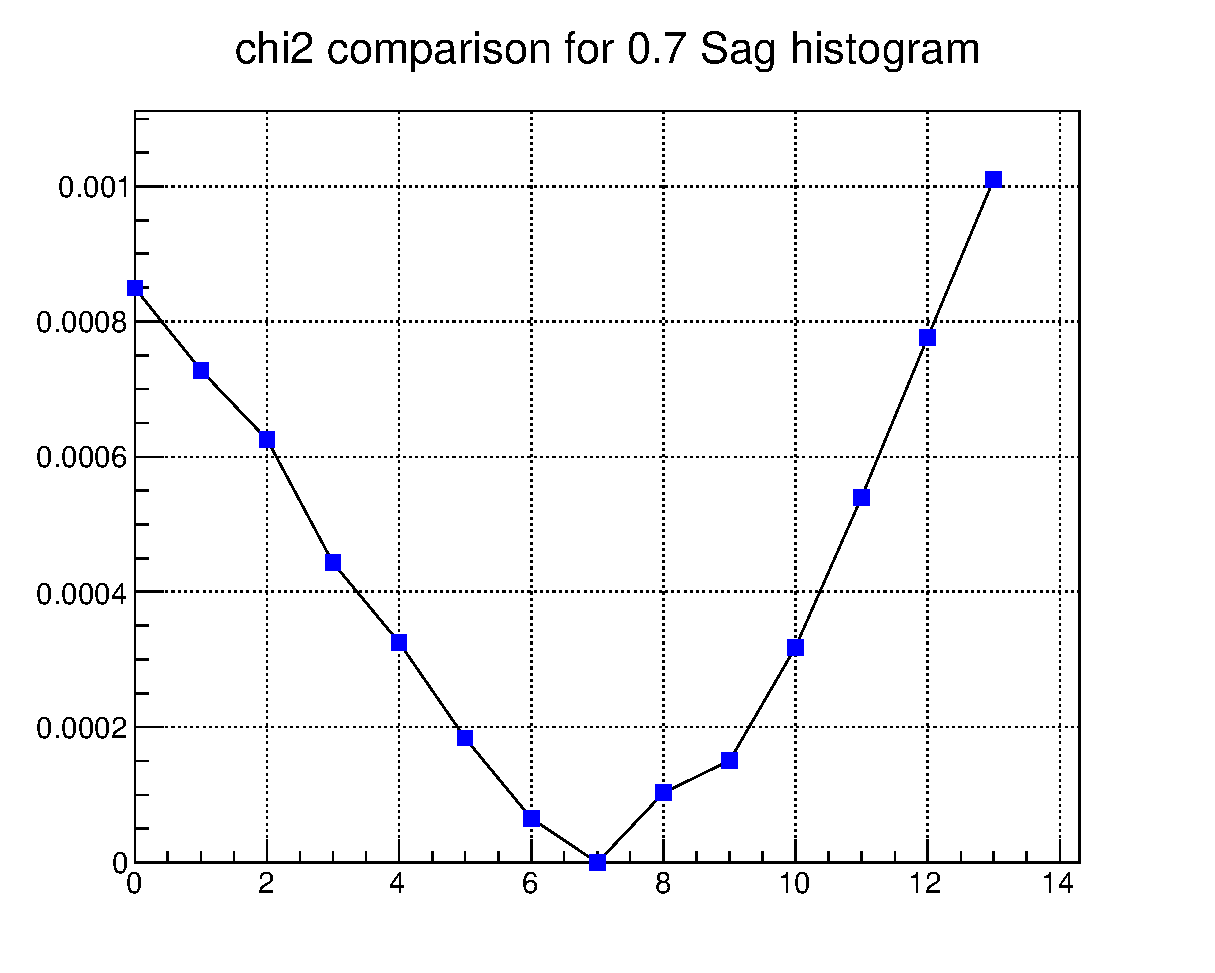
\includegraphics[width=0.45\textwidth]{chi2_07} 
			\label{fig:chi2for07} }%
		\qquad
		\subfloat[ Distribution of wire offset reconstruction from 180 series 5k events each. 50k events for $core$ template histograms. True bias is $0.063 mm$. 1 bin = 0.1 mm.]{
			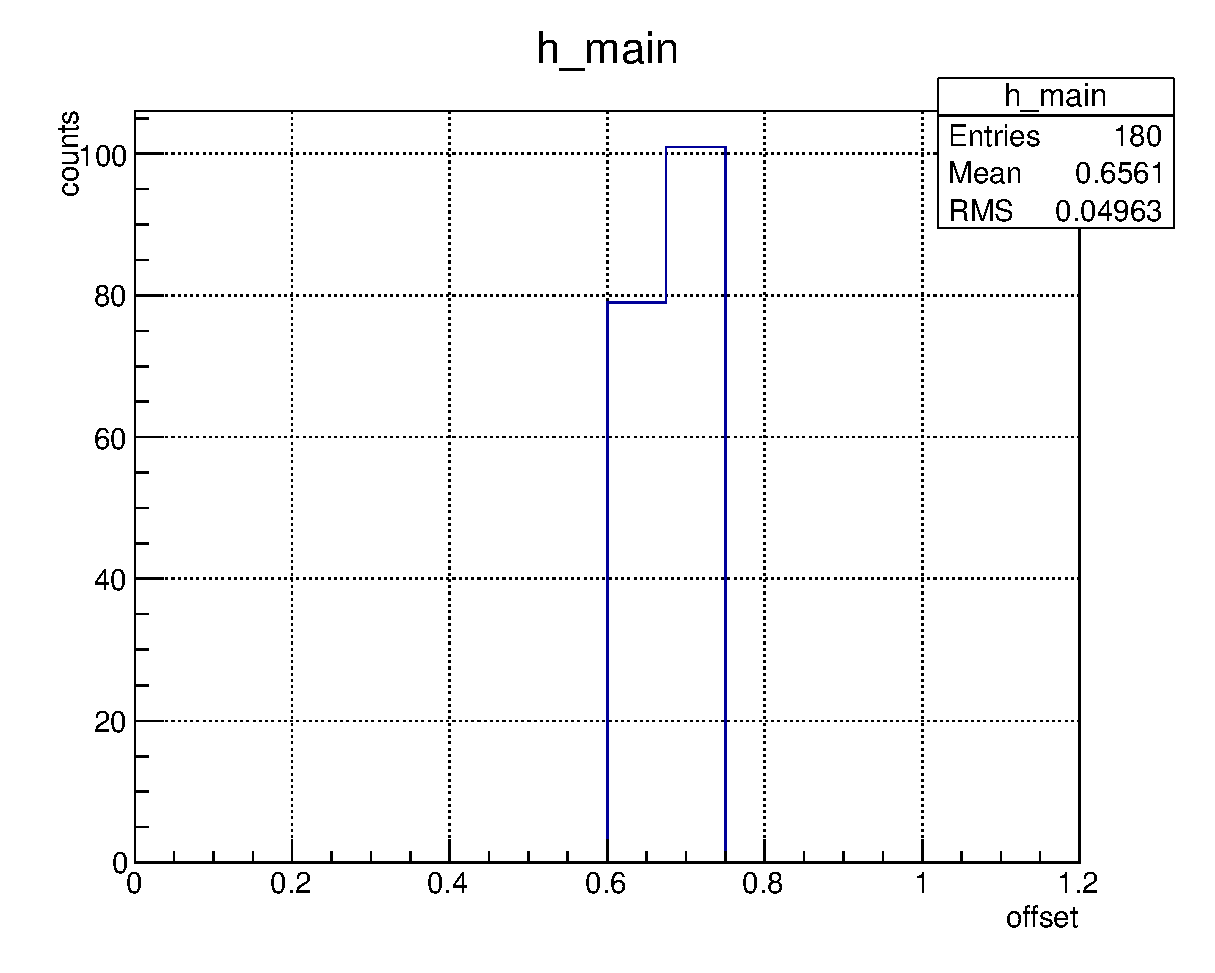
\includegraphics[width=0.45\textwidth]{chi_063_5k} 
			\label{fig:chi_063_5k} }%
		\caption{Wire position(offset) reconstruction}			
	\end{figure}	

	
	On the figure \ref{fig:chi_063_5k} you can see distribution wire sag calculation for 180 histograms with 5k events statistic. Precision in this case  $\sim 50\mu$. The algorithm of sag estimation is pretty simple: wire offset value eual to the as best match between $test$ and $core$ histogram.

	After we know sag value at some points of the tube or every where we can make one awesome collective analysis. The smoothing of wire offset value along the tube will give us much more precision results.  Fitting of sag value at  every point of $s(l)$ by some parabolic function should provide us the best results.
	
	\textcolor{red}{ Here i would like to put total plot of wire sag profile and compare reconstructed profile with true profile.}
	
	
	\section{Track reconstruction}
	
	The time between the track hit time stamp and the signal rising edge is a measure of {\it drift time} of these electrons. The relation between the   {\it drift time} and  the distance from the track to the center of the tube(wire while no sag for centered wire) is called {\it drift time - distance relation} or {\it tr-relation}.
	
	The drift time $t$ is a function of track position relative to the wire(so it's means the track position) and electric field along the drift trajectory.
	
	Assumed that the working  position  for straws will be parallel to the particle bunch, and  acceptance of particle spreading will not be significantly big. So tracks will be collinear each other within every separate  STRAW tube unit.
	
	Summing the above mentioned we have one dimension task -- reconstruct tracks on vertical axis\footnote{An example of single track reconstruction which explains the approximate procedure of reconstruction you can see on Fig.\ref{fig:track_reconstruction}}	(see examples of outcome tr-distribution $t = t(r,s=0)$ in Fig.\ref{fig:t_r_distr_00} and Fig.\ref{fig:tr_distr_15})  even the wire sagging. Sagging will be always down thanks to gravitation force $\vec{g}$.
	
	\begin{figure}[h!]
		\centering
		\subfloat[wire at the center]{
			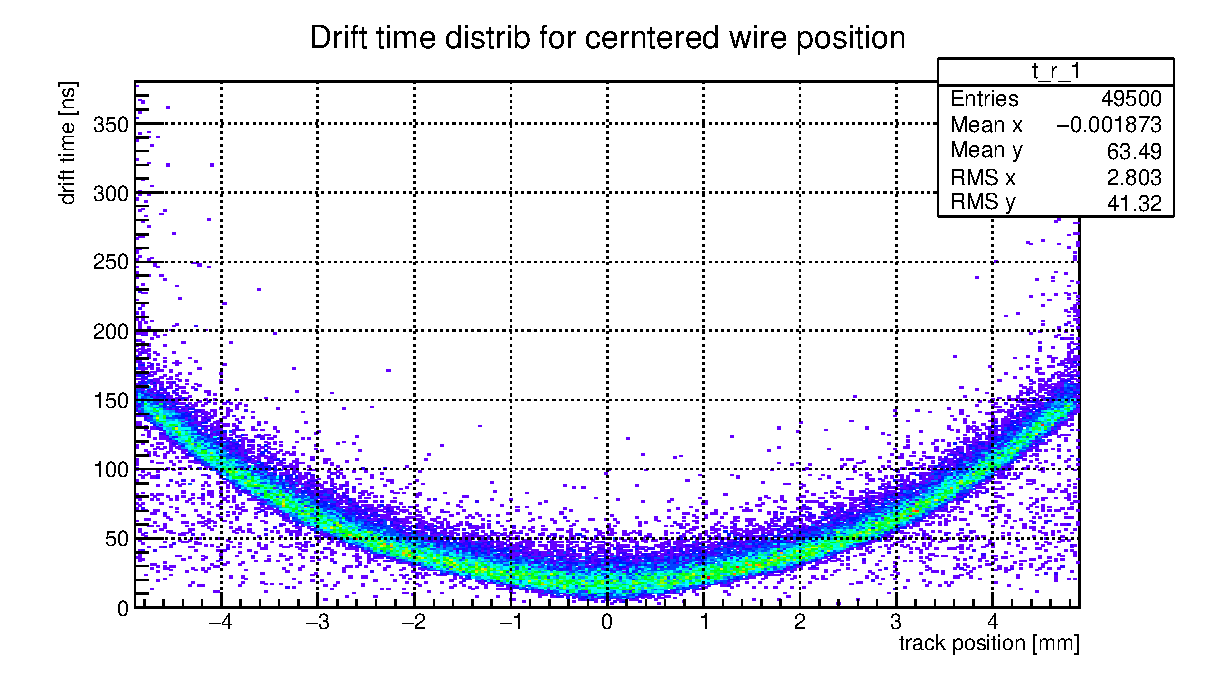
\includegraphics[width=0.45\textwidth]{t_r_distr_00} 
			\label{fig:t_r_distr_00} }%
		\qquad
		\subfloat[$1.5mm$  offset]{
			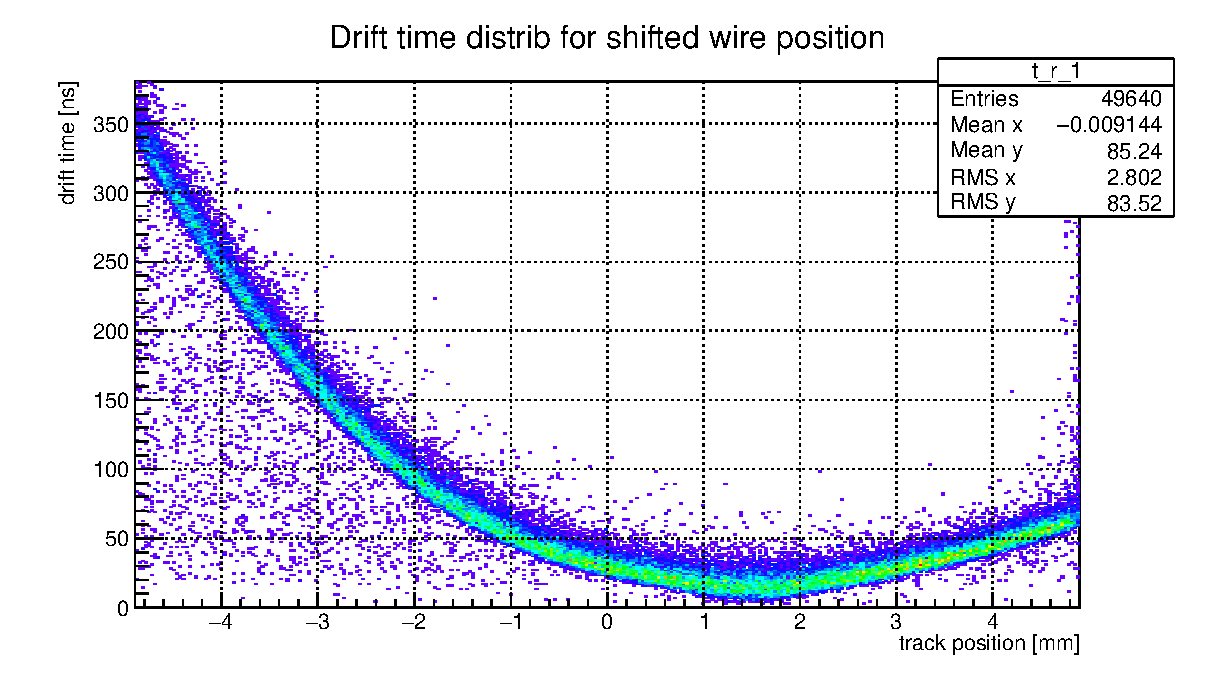
\includegraphics[width=0.45\textwidth]{tr_distr_15} 
			\label{fig:tr_distr_15} }%
		\caption{Distribution of drift time $t_{drift}$ as function of track position $r_{track}$ relatively to the tube center}			
	\end{figure}	
	
	The rt-relation is differ along the tube because different wire position $s$. Thus we have for the drift time 
	\begin{equation}
	t_{drift} = t_{drift}(r_{track},s)
	\end{equation}
	
	The idea to STRAW tube is to find the inverse dependence
	\begin{equation}
		r_{track} = r_{track}(t_{drift},s)
	\end{equation}
	
	From the section "Sag estimation" we can find sag profile for straw. Therefore the rt-calibration becomes 1 dimension less:
	\begin{equation}
		r = r(t,s=const)
	\end{equation}
	
	
	\subsection{How drift time resolution depend on wire offset?}
	
	Distorting of electric field inside the tube invoked by wire displacement from the center position will make an effect on drift time. Here we are going to estimate magnitude of drift time change.
	
	As was noted above we make a binning  for our data along the $r_{track}$(fig. \ref{fig:t_r_distr_00}, \ref{fig:tr_distr_15}). The resolution at every bin  is RMS of every bit digram (fig.\ref{fig:driftTimeResolutionEvo}).
	
	\begin{figure}[h!]
		\centering
		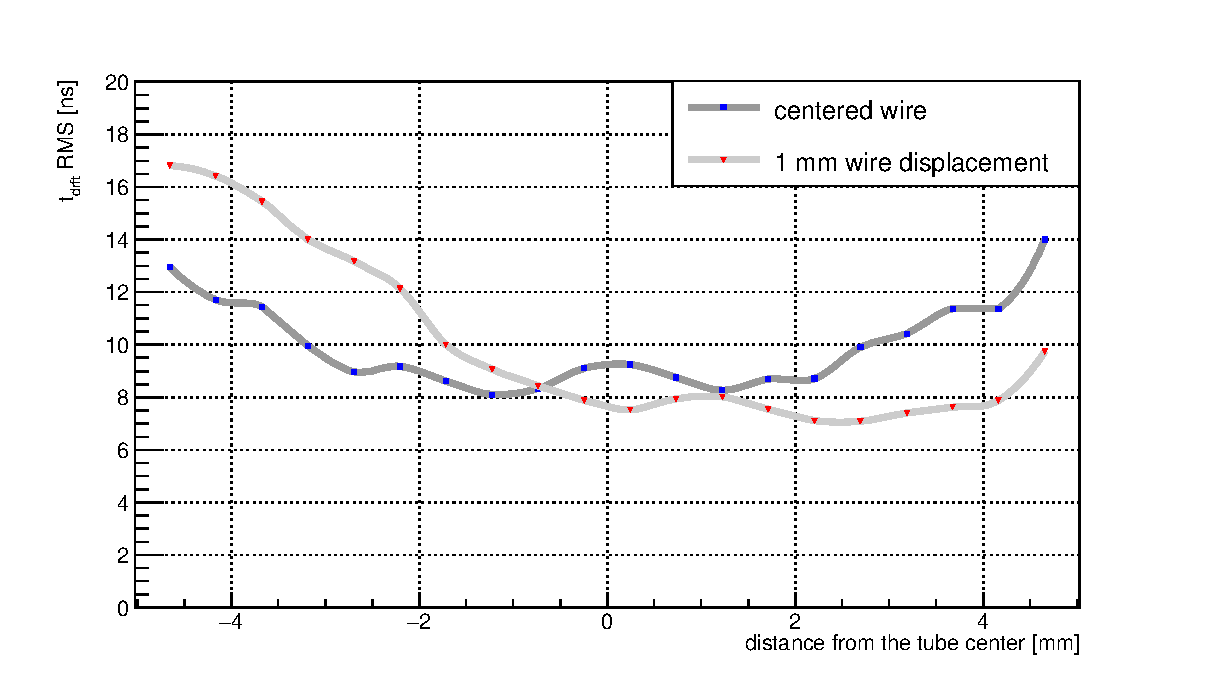
\includegraphics[width=0.9\textwidth]{DTimeRMS2}
		\label{fig:driftTimeResolutionEvo}
		\caption{Resolution of drift time as a function of distance from the wire.}
	\end{figure}
	
	We are dealing with probabilistic  nature of clustering that spread rt-relation from thin line. The leakage noise is also present in calculation but the effect of it i snot very high(especially in this calculation).
	
	Every plot of output current (see fig. \ref{fig:signal_example}) consist of 1000 equidistant frames. The threshold is set to $5\sigma$ of noise. Leakage nose make effect on drift time measurements in case its amplitude becomes higher that threshold value in range from $t=0$ to $t= t_{drift}$. At five-sigma there is only one chance in nearly two million that a random fluctuation would yield the result. The drift time for tracks close to the tube edge can be up to $150 ns$ and $300 ns$ in case wire displaced. The probability to meet noise above threshold value is less than $0.02\%$.
	
	Another source of noise points on tr-distribution comes from $\delta$-electrons that cause secondary ionisation in tube volume. The impact do only those electrons which are emitted in the direction of the wire(see example on fig.\ref{fig:deltaElectron}).
	
	\begin{figure}[h!]
		\centering
		\subfloat[$\delta$-electron affects on drift time]{
			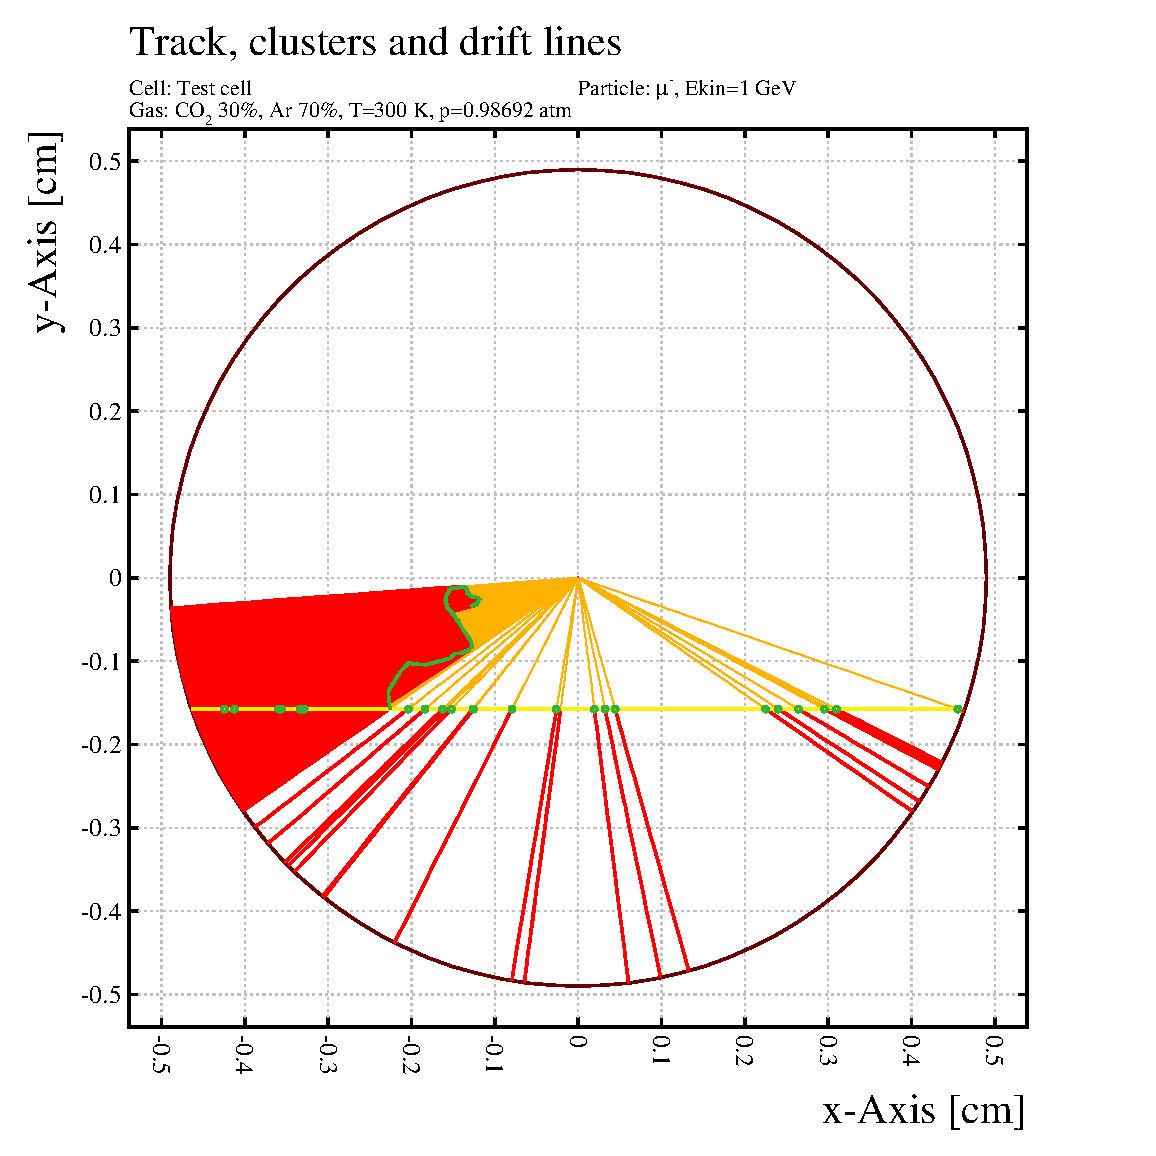
\includegraphics[width=0.45\textwidth]{deltaElectron} 
			\label{fig:deltaElectron} }%
		\qquad
		\subfloat[$\delta$-electron that moves away from the wire has no affect on drift time]{
			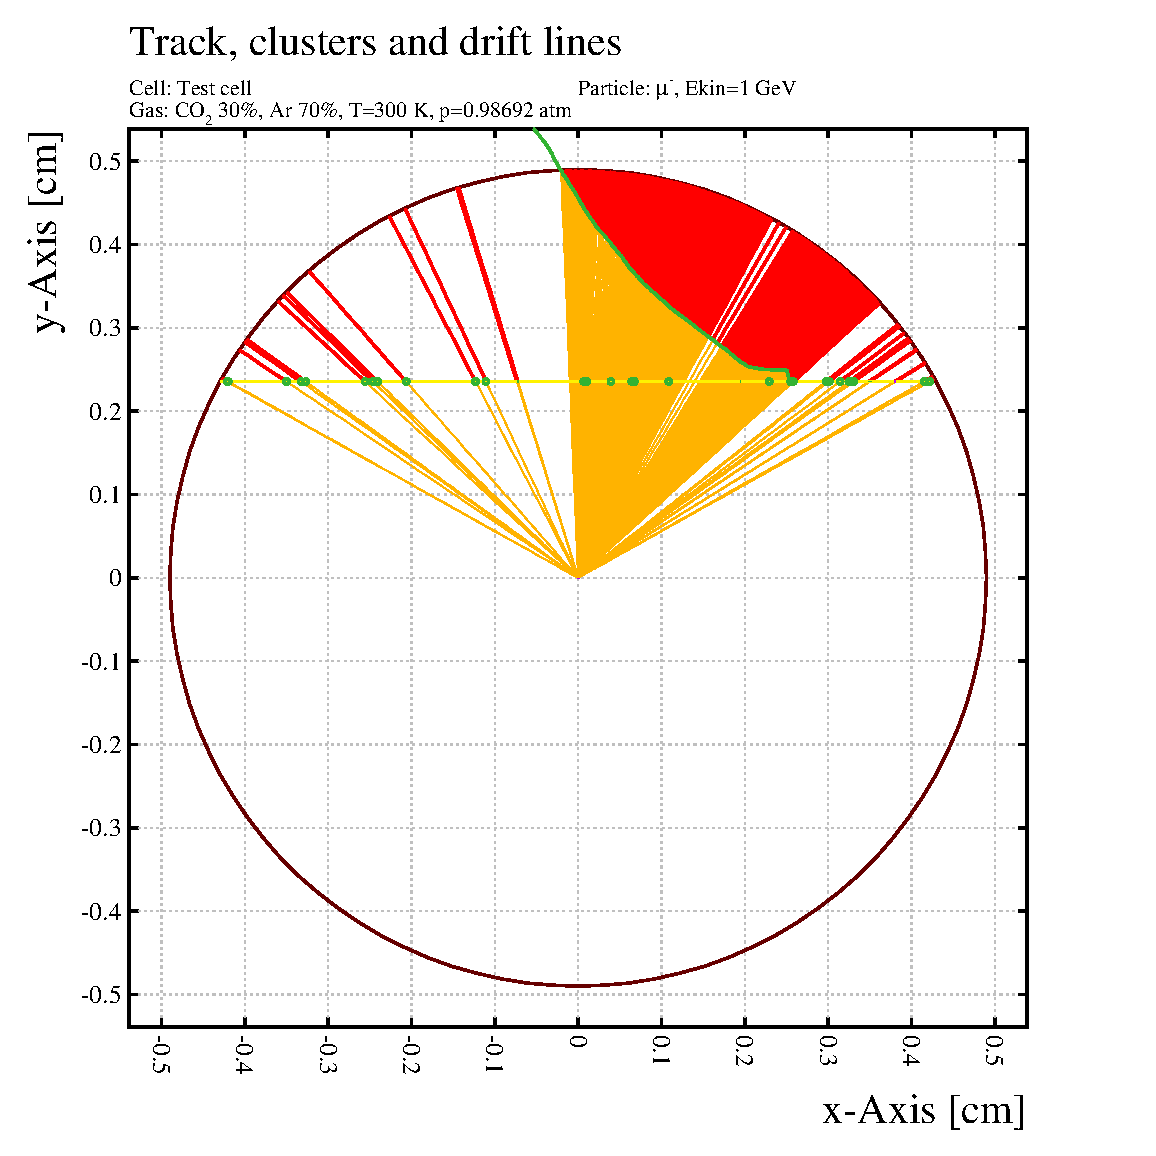
\includegraphics[width=0.45\textwidth]{deltaElectronNoEffect} 
			\label{fig:deltaElectronNoEffect} }%
		\caption{Garfield simulation with $\delta$-electron presence. Red lines - ion trajectory, yellow - electrons. Trajectory of $\delta$-electron marked by green curve line.}			
	\end{figure}	
	
	The number of events out of TR-ralation because of $\delta$-electrons is quite small. Especially percentage of events where $\delta$-electrons make effect on drift time is less that $1\%$ of total number of events  in GARFIELD simulations. 
	
	Tube wall is very thin but particle still can cause $\delta$-electrons when crossing it. GEANT4 studies show that such kind effect also presents in interaction of muon with tube volume, and percentage of events with $\delta$-electron that affect drift time even less that $0.2\%$.
	
	\subsection{Finding of rt-relation}
	
	The rt-relation depict relation between drift time and track position. The idea is to find the best fit of give data to achieve higher resolution and avoid systematic errors.
	
	The problem that we have to minimize influence of noise while fit. One suppose that the noise have approximately homogeneous distribution of points that locates below the main line of distribution. Consequently we can filter it by fitting only points from regions with local point density higher that some threshold value. Another way is to make a binning our distribution along the track position and fit every 1-D histogram by Gaussian. The fit points of Gaussian mean values by fit function.    
	
	Nevertheless our data contain very small amount of "non-track" points.
	
	TR-relation is asymmetry relatively to the $r=0$ almost in all cases except wire in the center of the tube. Therefore we have to calibrate for every of branches. It means we need to find two track positions for every of drift time value and reject one of them in further data processing stages.
	
	In previous section we found way to measure wire sag profile. So we can use this trick in present stage for separating data into ``right'' and ``left'' branch. Every of branches we will calibrate separately.
	
	Lets suppose we can fit every of tr-diagram by pair of analytic fit function (\ref{eq:trRelation}):
	\begin{equation}
	t(r_{track}) = e^{a_0 + a_1r_{track}}
	\label{eq:trRelation}
	\end{equation}
	
	\begin{figure}[h!]
	\centering
	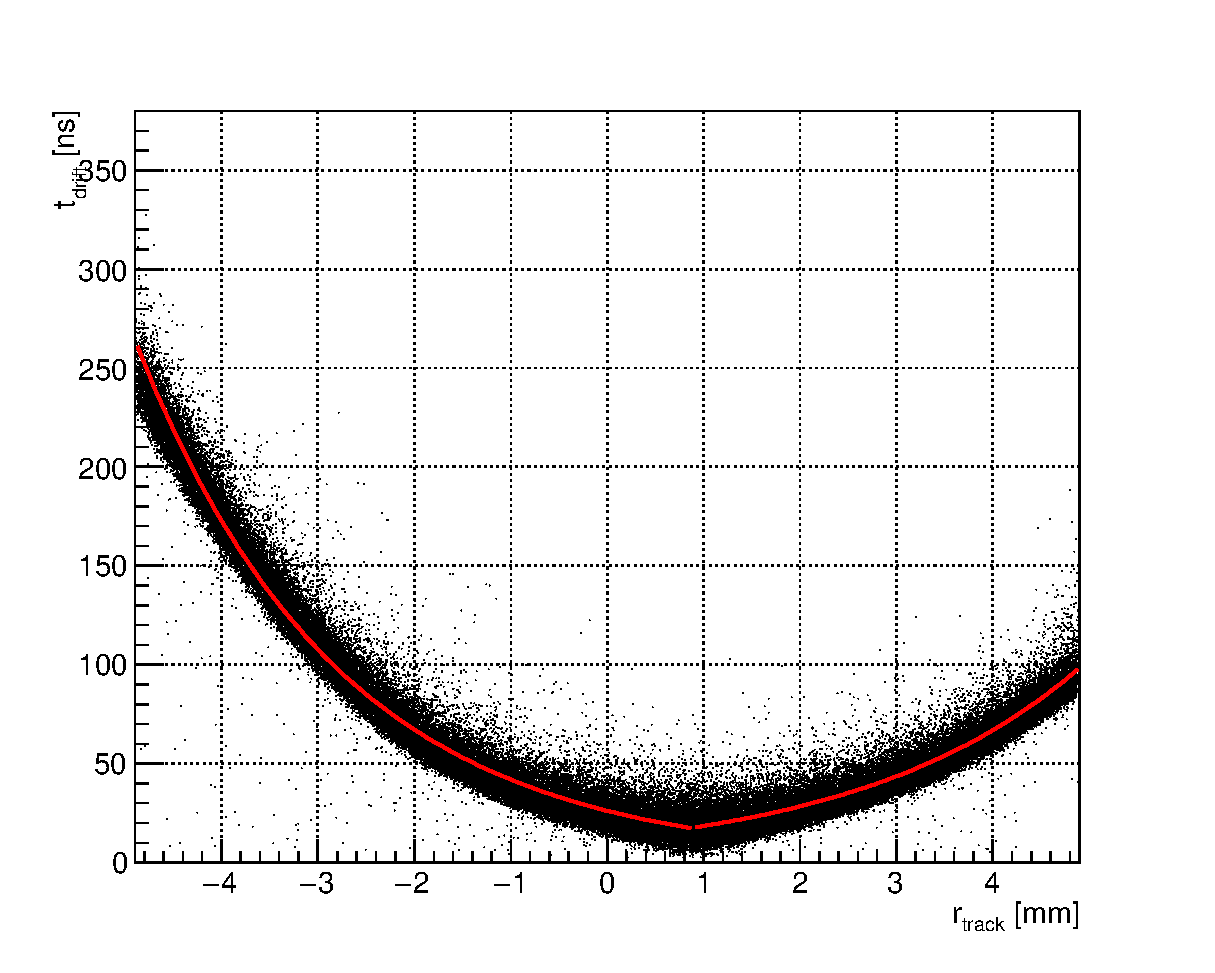
\includegraphics[width=0.7\textwidth]{TRrelation_09_points}
	\label{fig:TRrelation09points}
	\caption{TR-relation fitting for $0.9 mm$ wire offset value}
	\end{figure}
	
	If the figure \ref{fig:TRrelation09points} you can see tr-relation. Fitting is not perfect because of using simple fit function template (\ref{eq:trRelation}). But we will use reverse to the (\ref{eq:trRelation}) relation, because we have to find $r_{track}$ from known $t_{drift}$. We can do it be because the aim of this studies is not a precision calibration but global evaluation affect of wire sagging into total result.
	
	As you can see in the figure \ref{fig:TRrelation09points} red fit line does not cover whole drift time spectre. So events with drift time less than covered range(less than $\sim20 ns$) counts as track through the wire:
	\begin{equation}
	r_{track}(t_{drift} < t_{min}) = r_{wire~pos}
	\end{equation}
	where $t_{min} = min (t_{drift}(r_{track}))$, $r_{track} = \overline{(-r_{tube},r_{tube})}$. Respectively tracks with drift time higher than maximum of fit function range artificially counts as tracks with near tangents to the tube position $r_{track} = \pm r_{tube}$  (because efficiency decreases near the tube wall down to $20\%$).
	
	\subsection{Track reconstruction precision}
	
	Obviously precision is head factor when during we decide design of detector.
	
	The STRAW tube tracker should be as light as possible to avoid multiple scattering on structural components of detector. But design should be changed within reason if precision suffers from this\footnote{Especially design with no sagging works well for experiment NA62 \cite{}. But they have more than 2 times shorter  straw when tube have insert in the middle of the tube. So sagging becomes negligible in this case.}.
	
	How precision of track reconstruction depends on wire position(wire displacement)?
	
	\begin{figure}[h!]
		\centering
		\subfloat[reconstructed track position $r_{rec}$ as function of true track position $r_{track}$]{
			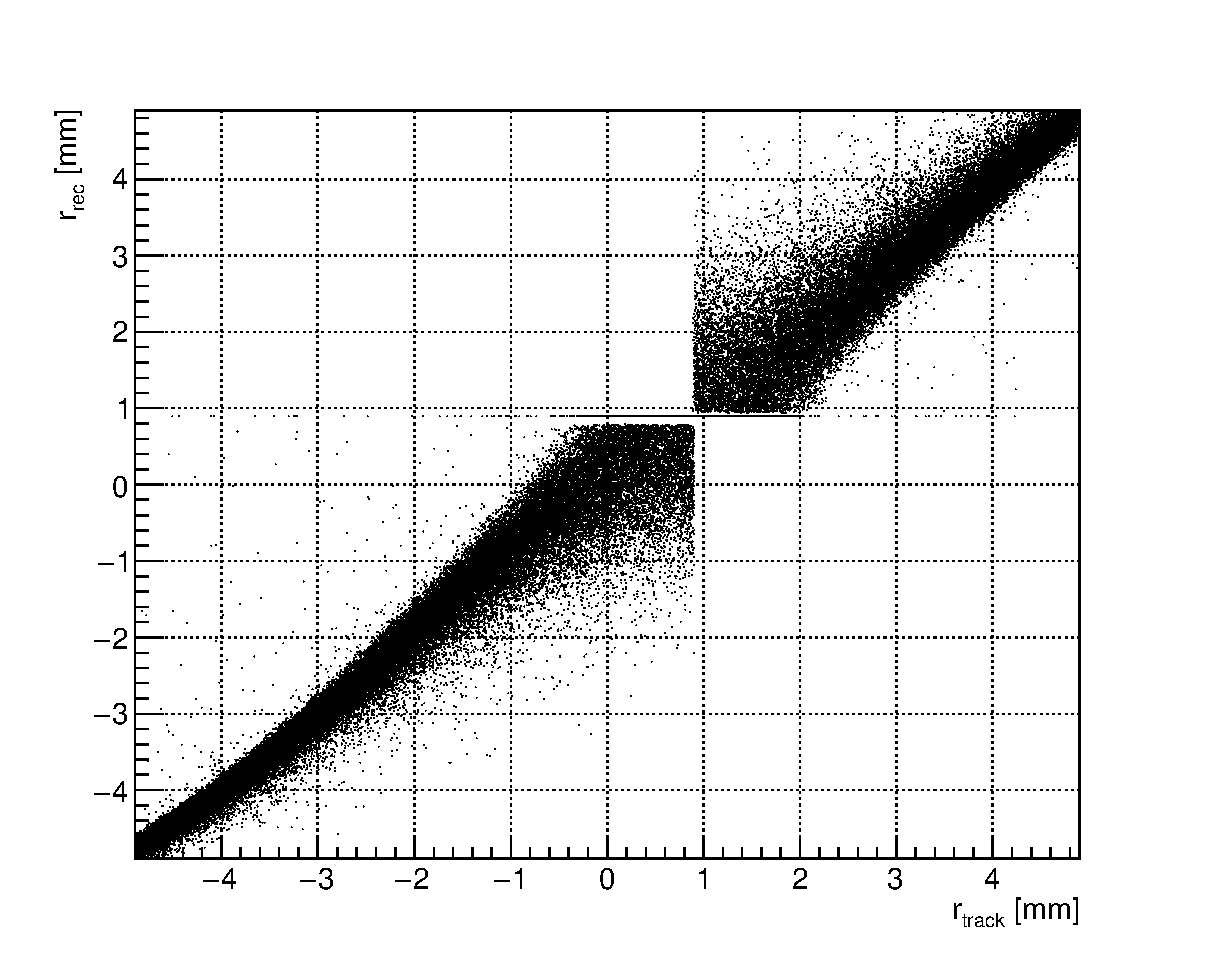
\includegraphics[width=0.4\textwidth]{reconstructed_points} 
			\label{fig:reconstructed_points} }%
		\qquad
		\subfloat[$r_{track} - r_{reconstructed}$ as function of $r_{track}$]{
			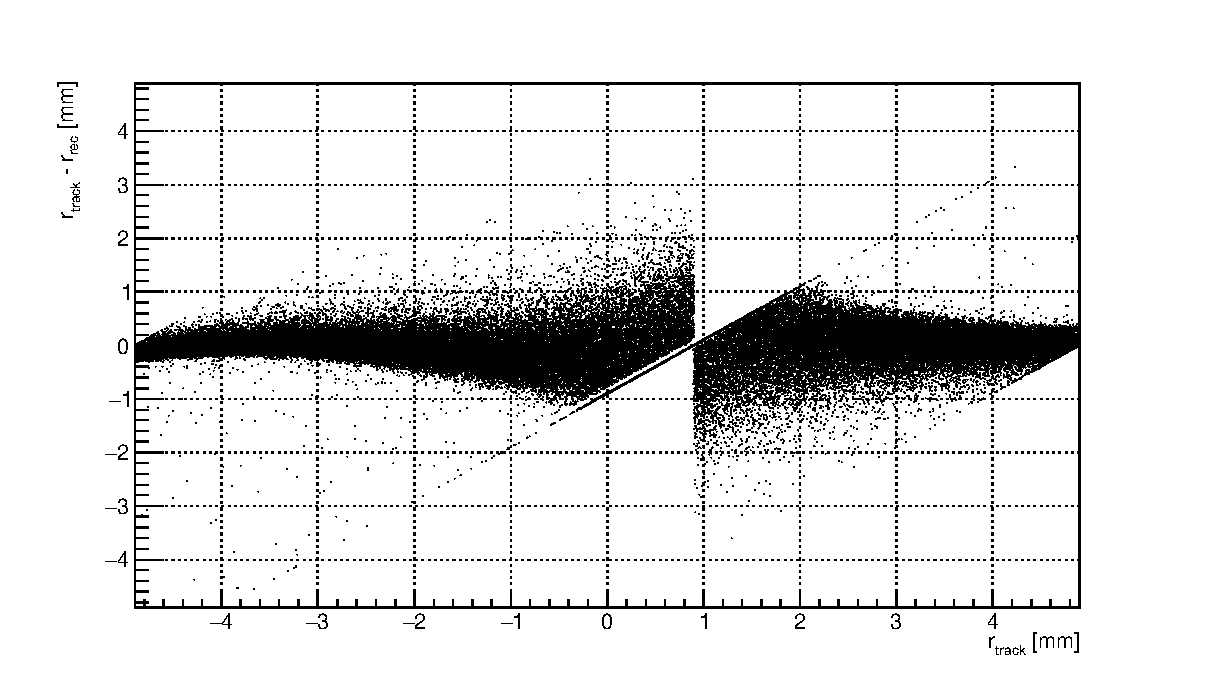
\includegraphics[width=0.5\textwidth]{diffRecTrue09_points} 
			\label{fig:diffRecTrue09_points} }%
		\caption{Distributions of matching of track position to their reconstructed value.}
	\end{figure}
	
	\begin{figure}[h!]
	\centering
	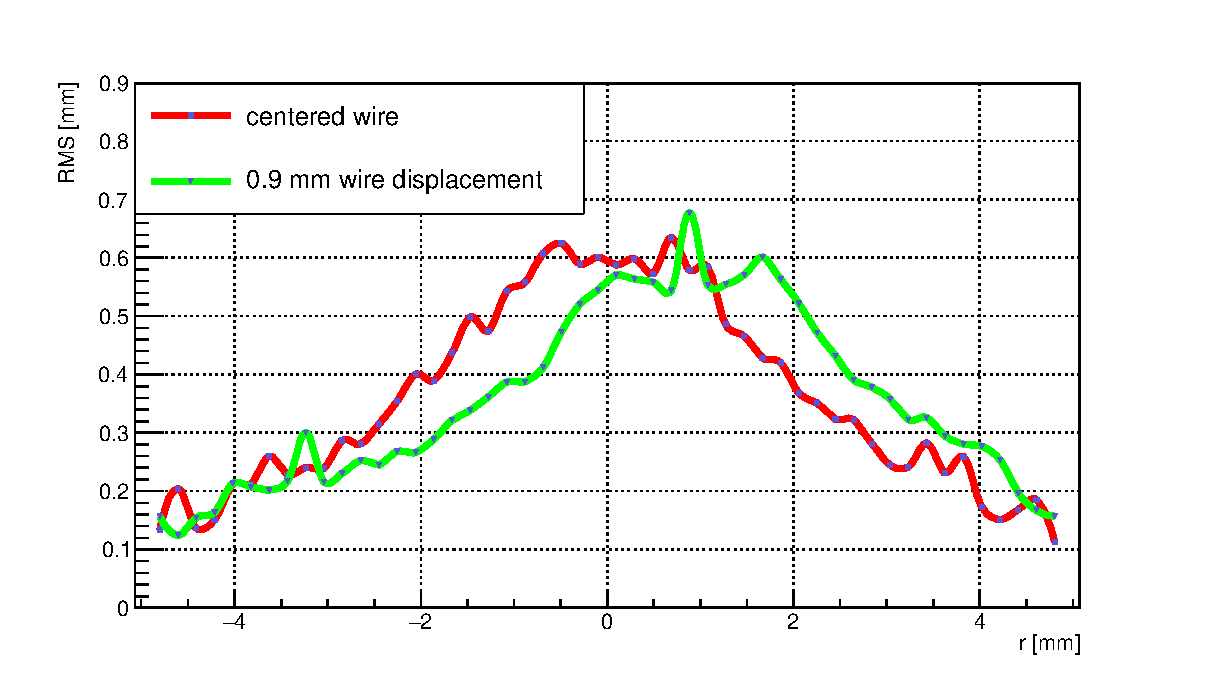
\includegraphics[width=0.9\textwidth]{precisionCompare_0_9}
	\label{fig:precisionCompare09}
	\caption{Comparison of track reconstruction precision for two wire position. Value of precision at every point means RMS of data sample near corresponding track position $r$. Red line corresponds to the centered wire position, green line -- to the $0.9 mm$ sagged wire  position.}
	\end{figure}
	
	As you can see on figure \ref{fig:precisionCompare09} there are no significant difference of track reconstruction precision between two mode of wire location despite of the increasing drift time for displaced wire position(with almost factor of two).	 The highest resolution($\sim 0.1 mm$) near the tube wall and worst value $\sim0.6mm$ is near the wire because the clustering effect. Higher gas pressure should resolve this problem.
	
	\subsection{Порівняння розподілів для центрального та зміщеного позицій дроту в трубці}
	Наведемо порівнняння гістограм для центрального та зміщеного позицій дроту для вибірки треків в околі дроту та на відстані 2 мм від нього.
	
	\begin{figure}[h!]
	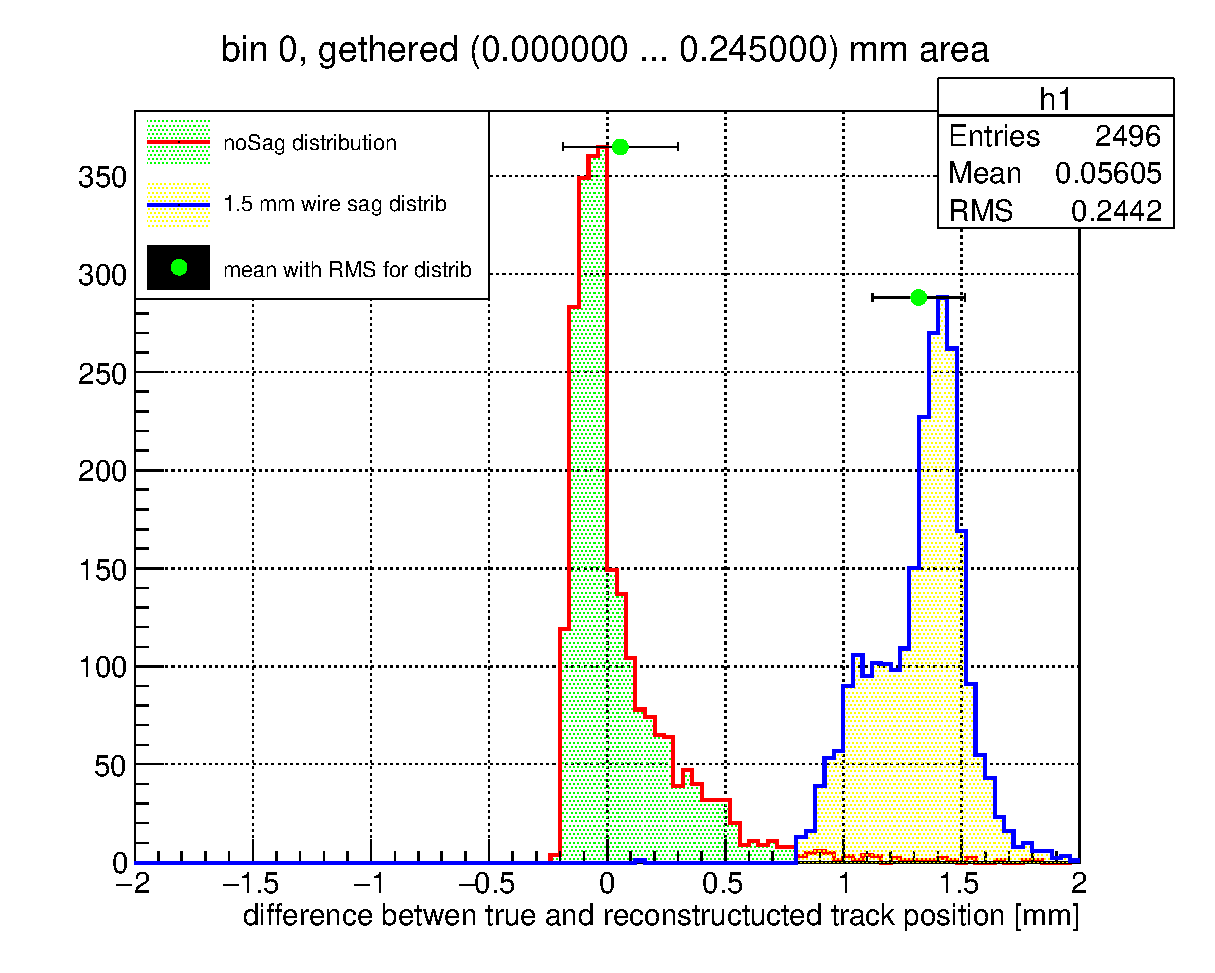
\includegraphics[width=0.8\textwidth]{bin0_0mm.eps}
	\centering
	\caption{ Порівняння розподілу реконструкції позицій треків для центрального положення дроту та вападку зміщення дроту дрейфової трубки на $1.5 mm$ від центрального положення для треків які проходять близько до центру трубки}
	\end{figure}
	
	\begin{figure}[h!]
	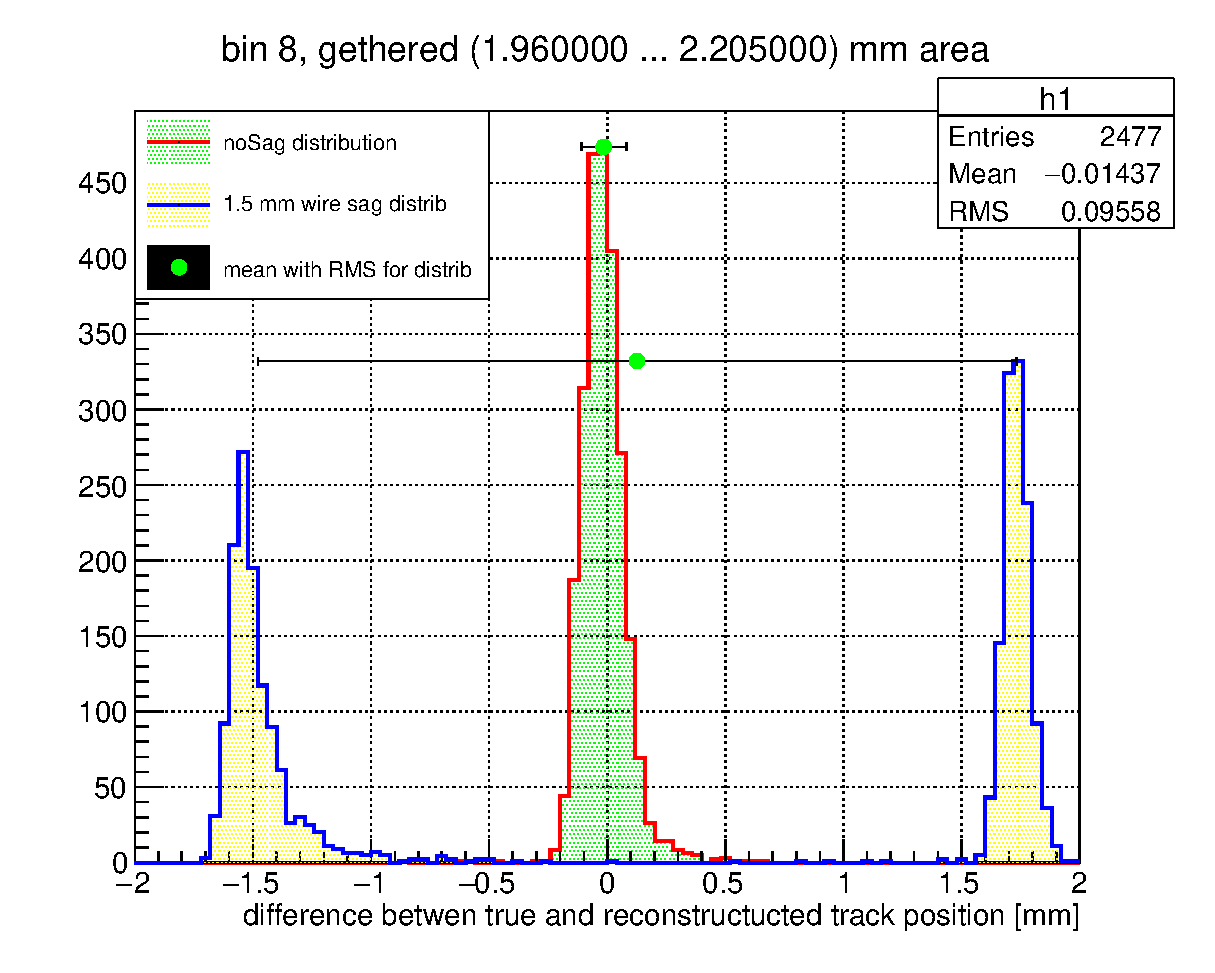
\includegraphics[width=0.8\textwidth]{bin8_2mm.eps}
	\centering
	\caption{ Порівняння розподілу реконструкції позицій треків для центрального положення дроту та вападку зміщення дроту дрейфової трубки на $1.5 mm$ від центрального положення для треків які проходять дотично до кола радусом $2mm$  коцентричного з трубкою}
	\end{figure}
	
	Цілком логічно припускати, що електроніка реєструватиме час дрейфу відмінний від триманого нами від симуляцій описаних вище. Тож необхідним буде врахувати внесок від електроніки. Ситуація ускладнюється тим що окрім форми вхідного сигналу потрібно знати ще й амплітуду сигналу(сумарний заряд зібраний з треку з урахуванням підсилення).
	
\newpage
\begin{thebibliography}{00}
	\bibitem{garfield} http://garfield.web.cern.ch/garfield

	\bibitem{kozlinskiy}  thesis Kozlinskiy.pdf 
	
\end{thebibliography}
	
\end{document}